% **************************************************
% Document Class Definition
% **************************************************
\documentclass[%
    paper=A4,               % paper size --> A4 is default in Germany
    twoside=true,           % onesite or twoside printing
    openright,              % doublepage cleaning ends up right side
    parskip=half,           % spacing value / method for paragraphs
    chapterprefix=true,     % prefix for chapter marks
    11pt,                   % font size
    headings=normal,        % size of headings
    bibliography=totoc,     % include bib in toc
    listof=totoc,           % include listof entries in toc
    titlepage=on,           % own page for each title page
    captions=tableabove,    % display table captions above the float env
    chapterprefix=false,    % do not display a prefix for chapters
    appendixprefix=false,    % but display a prefix for appendix chapter
    draft=false,            % value for draft version
]{scrreprt}%


% **************************************************
% Setup YOUR thesis document in this file !
% **************************************************
\input{my-thesis-setup}


% **************************************************
% Document CONTENT
% **************************************************
\begin{document}

% uncomment the following command to fill up pages with
% whitespace instead of aligning the first and last lines
% of a page (see \raggedbottom vs. \flushbottom)
%\raggedbottom

% --------------------------
% rename document parts
% --------------------------

% > set short label names for floating environments figure and table
%\renewcaptionname{ngerman}{\figurename}{Abb.}
%\renewcaptionname{ngerman}{\tablename}{Tab.}
\renewcaptionname{english}{\figurename}{Fig.}
\renewcaptionname{english}{\tablename}{Tab.}

% > rename the title of the LOL, i.e. list of listings (default is "Listings")
\renewcommand*{\lstlistlistingname}{List of Listings}

% --------------------------
% Front matter
% --------------------------
\pagenumbering{roman}			% roman page numbing (invisible for empty page style)
\pagestyle{empty}				% no header or footers
\input{content/titlepages}		% INCLUDE: all titlepages
\cleardoublepage

\pagestyle{plain}				% display just page numbers
\input{my-content/abstract}		% INCLUDE: the abstracts (english and german)
\cleardoublepage
%
% !TEX root = ../my-thesis.tex
%
\pdfbookmark[0]{Acknowledgement}{Acknowledgement}
\addchap*{Acknowledgement}
\label{sec:acknowledgement}

First and foremost, I want to thank Prof. Dr. Elmar Schömer and Dr. Rainer Erbes for being my supervisors during the writing of this thesis. They are always able to move their students in the right direction and are ready to help where help is needed.

I also want to thank Yan Chernikov, the creator of the YouTube channel \textit{TheCherno} where he uploads excellent videos on topics related to computer graphics and programming in general.
 % INCLUDE: acknowledgement
\cleardoublepage
%
\currentpdfbookmark{\contentsname}{toc}
\setcounter{tocdepth}{2}		% define depth of toc
\tableofcontents				% display table of contents
\cleardoublepage

% --------------------------
% Body matter
% --------------------------
\pagenumbering{arabic}			% arabic page numbering
\setcounter{page}{1}			% set page counter
\pagestyle{scrheadings}			% header and footer style

$$
\rho(\textbf{r}) = \int_{\mathbb{R^3}}  d \textbf{r}
$$

%% !TEX root = ../my-thesis.tex
%
\chapter{Related work}
\label{sec:related}

Particle-based approaches to fluid dynamics have made an extensive evolution during the last decades. Researchers had moved from rendering particles as spheres to fluid mesh extraction using for example an algorithm called marching cubes \cite{Muller:2003, Williams:2008, Yu:2013}. But with GPUs becoming more and more powerful, screen-space techniques for rendering particle-based fluids - like the one discussed in this thesis - have emerged and gained popularity \cite{Wu:2022, VanDerLaan:2009}. The core difference to traditional methods is that the surface extraction happens for every pixel of the screen. Thus, only the visible parts of the fluid are actually computed and the rendered image is of high quality due to the fine details that can be extracted at the pixel-level.

There are countless papers introducing new techniques for rendering different parts of a fluid. Ihmsen et al. \cite{Ihmsen:2012} for example propose a method for rendering foam and bubbles at wave crests.

Particle-based fluid simulation has even made its way into deep learning with Ummenhofer et al. \cite{Ummenhofer:2020} among others developing a neural network that can predict new particle positions from the previous simulation step.

%% !TEX root = ../my-thesis.tex
%
\chapter{Introduction}
\label{sec:intro}

The primary source of this thesis is the paper \textit{A Real-Time Adaptive Ray Marching Method for Particle-Based Fluid Surface Reconstruction}, written by Tong Wu, Zhiqiang Zhou, Anlan Wang, Yuning Gong and Yanci Zhang. In addition to reformulating its contents, we introduce details about our implementation to further build an understanding of the authors' work and to supply anchor points for anyone attempting to develop an implementation for their own.

Williams \cite{Williams:2008} states that computational fluid dynamics consists of three phases: simulation, extraction of a renderable representation, and rendering itself. This work focuses on the latter two. The authors of our primary source build on top of existing advancements in the field and propose algorithms and data structures that aim to make those methods capable of running in real-time.

Whenever we write "the authors" or "Wu et al." we are referring to ideas coming from our primary source. We distinguish between our and others' thoughts by mentioning their origin. Unfortunately, we did not have the time to implement every aspect of the authors' algorithm. Details on the parts we implemented can be found in the \textbf{Implementation} subsections of each chapter.

\section{Structure}

We will start by establishing some notation and explain the reasoning behind our choices regarding implementation details like programming language and libraries. Then we will introduce the theoretical backbone behind particle fluid simulation in \textbf{Smoothed Particle Hydrodynamics \myref{sec:sph}}. Since there are many parts to the described algorithm that have to be addressed, we will give a broad overview in the section \textbf{Pipeline overview \myref{sec:pipelineoverview}} before going into more depth explaining all steps necessary for displaying a fluid on screen. Finally, we will present our results by showing screenshots of our application together with some measurements that qualify the different techniques applied.

\section{Technology}

We decided to use C++ together with \textit{Vulkan} as our graphics API. \textit{Vulkan} is a state-of-the-art graphics API allowing for very low-level access to GPU processes and resources. Although this is not strictly necessary for the application discussed here, learning about \textit{Vulkan} is as interesting as it is useful for moving deeper into graphics programming, which is why we chose to use it. \textit{Vulkan} opens the door to vast improvements in computation time by letting the user decide which computations should run in parallel, what memory is accessible where, and much more. By leveraging more of \textit{Vulkan}'s features, the computation time needed by our implementation could reduce by orders of magnitude. These possibilities are discussed further in the chapter \textbf{Future work \myref{sec:futurework}}.

Other libraries that were used are listed here, some of which are described in more detail later:
\begin{enumerate}
    \item \textit{Dear ImGui} for the graphical user interface \cite{ImGui}
    \item \textit{GLFW} for window management
    \item \textit{Partio} for importing particle data \cite{Partio}
    \item \textit{Eigen} and \textit{glm} for math \cite{Eigen}
    \item \textit{CompactNSearch} for neighborhood search \cite{CompactNSearch}
    \item \textit{SPlisHSPlasH} for dataset generation \cite{SplishSplash}
\end{enumerate}

The code for our implementation can be found on GitLab (\url{https://gitlab.rlp.net/leschere/bachelor-thesis}).

\section{Terminology}

This is a collection of mathematical notation and symbols we use throughout this thesis.

\textbf{Notation}:

\begin{itemize}
    \item Vectors and matrices are written in bold font. The names of vectors are in lower case and those of matrices are in upper case:
        \begin{itemize}
            \item $\textbf{r} = (x, y, z)^T \in \mathbb{R}^3$
            \item $\textbf{C} \in \mathbb{R}^{n \times m}$
        \end{itemize}
        
    \item $| \textbf{r} | := \sqrt{ \sum_{i=1}^n r_i^2 }$ is the $L^2$-norm of the vector $\textbf{r} = ( r_1, \dots, r_n )^T$.
    \item $|| \textbf{r} || := \frac{1}{|\textbf{r}|} \textbf{r}$ is the unit vector pointing in the same direction as $\textbf{r}$.
    \item $\tilde{\textbf{r}} \in \mathbb{R}^4$ is a four-dimensional homogenous vector corresponding to a three-dimensional position vector $\textbf{r}$. In computer graphics, homogenous coordinates are used to calculate the projection of three-dimensional objects to the two-dimensional screen.
    \item $[\textbf{r}]_i$ is the $i$-th entry of the vector $\textbf{r}$. This is to distinguish between element indices and other types of indices the vector inside the brackets could have.
    \item $[\textbf{C}]_{ij}$ is the entry in the $i$-th row and the $j$-th column of the matrix $\textbf{C}$.
    \item $\overline{\textbf{C}}$ is the adjugate of the matrix $\textbf{C}$
    \item $\textbf{r}^2 := \textbf{r}^T \textbf{r} = |\textbf{r}|^2$
    \item $\text{diag}(a_1, a_2, a_3) := \begin{pmatrix} a_1&0&0\\0&a_2&0\\0&0&a_3 \end{pmatrix}$
\end{itemize}

\textbf{Symbols}:

\begin{itemize}
    \item $h$: the particles' radius
    \item $R_{N}$: neighborhood radius
    \item $\textbf{G}_i$: characteristic neighborhood matrix of the particle $i$
    \item $\sigma$: the density threshold at which the fluid's surface is assumed
\end{itemize}

%% !TEX root = ../my-thesis.tex
%
\chapter{Fundamentals}
\label{sec:fundamentals}

This chapter aims to equip the reader with the mathematical and conceptual basics of particle-based fluid dynamics. We will introduce the underlying theory of Lagrangian fluid simulation and its physical relevance. Afterward, we explain how our representation of the fluid is generated and how it is stored in memory.

\section{Smoothed Particle Hydrodynamics}
\label{sec:sph}

The macroscopic real world we are seeing and experiencing every day is of continuous nature. Computers on the other hand are unable to capture this continuity reasonably. Thus, computer scientists have to invent ways of discretizing physical problems to be able to construct simulations for them. Smoothed Particle Hydrodynamics (SPH) is one such method of discretization. Originally invented for the simulation of gravitational systems in astronomy, it is now widely used in fluid simulation.

There are two prominent mathematical theories describing the computational simulation of hydrodynamics \cite{Monaghan:2005}: \\
In \textit{Eulerian} hydrodynamics, the fluid's properties are observed at fixed locations in space, usually arranged in a grid. This technique has built the foundation of computational fluid dynamics as we know it today. \\
In \textit{Lagrangian} hydrodynamics, the fluid's properties are carried through space by individual particles. These quantities are evaluated at the particles' freely moving positions instead of at fixed grid points.
Both methods are still in simultaneous use today as they differ in computational efficiency and physical accuracy. The choice of a best fit depends heavily on the application.

SPH belongs to the \textit{Lagrangian} category. The core idea is to approximate a continuous function $f$ with a finite set of particles $p_i$. Each particle consists of a position $\textbf{r}_i \in \mathbb{R}^3$ and an associated feature $f_i \in F$. Together, these form the set of particles $P := \{ p_i: i = 0,...,n-1 \}$ with $p_i := (\textbf{r}_i, f_i)$. Here, $F$ is a generic set of feature values that is dependent on the context of the problem. In the application discussed in this work, the feature of interest is the fluid's density. This can be represented by a scalar in $\mathbb{R}$, which is why we set $F := \mathbb{R}$. In other applications for example, it is common to see $F := \mathbb{R}^3$ and $f_i \in F$ to be interpreted as the particle's velocity (see Ummenhofer et al. \cite{Ummenhofer:2020}).

The continuous distribution of a feature in three-dimensional space is given by a function
\[
f: \mathbb{R}^3 \rightarrow F.
\]
Iterating over all particles $(\textbf{r}_i, f_i)$, $f$ can be approximated by the finite sum
\[
f(\textbf{r}) \approx \sum_{i=0}^{n-1} \space \frac{m_i}{\rho_i} \space f_i \space W(\textbf{r}_i - \textbf{r})
\]
where $W: \mathbb{R}^3 \rightarrow \mathbb{R}$ is called the \textit{smoothing kernel}, $\rho_i$ is the particle's density and $m_i$ is the particle's mass. In our case, the feature we are seeking to compute is the fluid's density $\rho$, so we set $f_i := \rho_i, \space i = 0,...,n-1$ and therefore - assuming all particles have identical mass $m$ - the equation simplifies to
\[
\rho(\textbf{r}) \approx m \sum_i W(\textbf{r}_i - \textbf{r}).
\]
Physically speaking, $\rho$ has the unit $\frac{\text{kg}}{\text{m}^3}$ meaning the kernel function $W$ has to have the unit $\text{m}^{-3}$.

\subsection{Surface definition}
\label{sec:surfacedefinition}

The fluid's surface $\mathcal{S}$ is defined as an iso-surface of the scalar field $\rho(\textbf{r})$. It is the set of all points where the evaluated density equals a constant we call $\sigma$:
\[
\mathcal{S} := \{ \textbf{r} \in \mathbb{R}^3 : \rho(\textbf{r}) = \sigma \}
\]
This definition is implied in algorithm 1 of Wu et al. \cite{Wu:2022} and is the basis for the surface extraction algorithm described later (see the chapter \textbf{Surface extraction with ray marching \myref{sec:surfaceextraction}}).

\subsection{Smoothing kernels}

\begin{figure}[h]
    \centering
    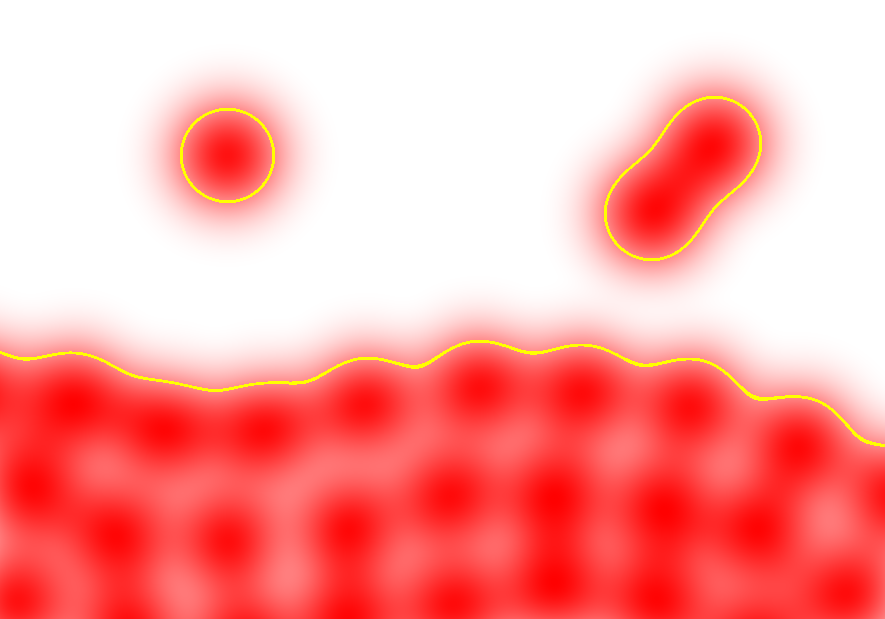
\includegraphics[width=0.75\textwidth]{my-gfx/figure-sph.png}
    \caption{An illustration showing how the kernel smoothes the particles' features across its neighborhood. The iso-surface $\mathcal{S}$ is indicated in yellow. The distinction between splash particles (top) and aggregated particles (bottom) can be seen and is important in later chapters.}
    \label{fig:sph}
\end{figure}

The kernel can be interpreted as a function that "smears" or smoothes the particles' features across space to create a continuum (see Figure \myref{fig:sph}). It must have some properties to function properly:

\begin{enumerate}
    \item Its volume integral over the entire domain is normalized (see \cite{Monaghan:2005}). This ensures that the kernel does not amplify the feature the particle is carrying:
    \[
    \int_{\mathbb{R}^3} W(\textbf{r}) \space d \textbf{r}' = 1
    \]
    
    \item It approaches the Dirac delta distribution for small support $h$ (explained below) (see \cite{Monaghan:2005}):
    \[
    \lim\limits_{h \rightarrow 0} W(\textbf{r}) = \delta(\textbf{r})
    \]
\end{enumerate}

For simulation, kernels are typically radially symmetric, meaning
\[ |\textbf{r}_1| = |\textbf{r}_2| \Rightarrow W(\textbf{r}_1) = W(\textbf{r}_2) .\]
However, this property is not always desired for this application for reasons explained in a later chapter.

The choice of a kernel function is important for error considerations and practicality. The authors did not state the specific function they used - only that it was a "symmetric decaying spline with finite support". In the following, the kernel definition by Koschier et al. \cite{Koschier:2019} will be used (see Figure \myref{fig:kernel}):

Let $r := \frac{|\textbf{r}|}{h}$:
\[
W(\textbf{r}) = c \frac{1}{h^3} P(r)
\]
where $c$ is a constant that satisfies the kernel's normalization constraint (for three dimensions $c := \frac{8}{\pi}$), $h$ is the particles' radius, and $P$ is a spline of the form
\[
P(r) = \begin{cases}
  6 (r^3 - r^2) + 1 , & 0 \leq r < \frac{1}{2} \\
  2 (1 - r)^3       , & \frac{1}{2} \leq r < 1 \\
  0                 , & \text{else.}
\end{cases}
\]
In this thesis, kernel functions $W$ are always understood with respect to the particle radius $h$ without stating so explicitly.

Note that this function is in fact radially symmetric, although we mentioned this to be an undesired property. It is used as the basis for a non-symmetric kernel later on.
These are some of the reasons for choosing this function:
\begin{itemize}
    \item It is simple and quick to compute.
    \item It has finite support, meaning $W(\textbf{r}) = 0, \forall \textbf{r}: |\textbf{r}| \geq h$. This opens the door for reducing the algorithm's time complexity, which is explained in the chapter \textbf{Particle neighborhood and anisotropic kernels \myref{sec:particleneighborhood}}.
\end{itemize}

\begin{figure}[h]
    \centering
    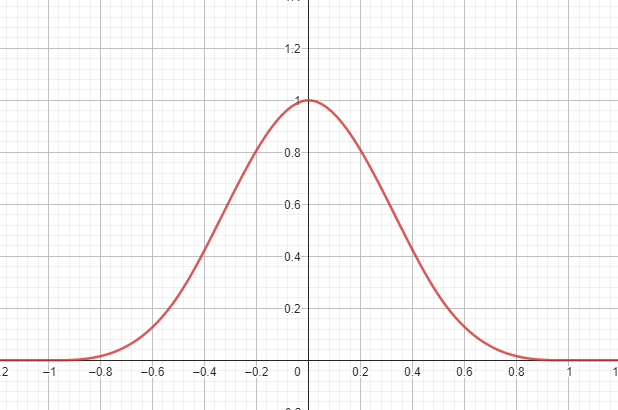
\includegraphics[width=0.75\textwidth]{my-gfx/figure-kernel.png}
    \caption{A graph showing the smoothing kernel we used. Here, only the spline $P$ is shown. The rest of $W$ consists only of scaling.}
    \label{fig:kernel}
\end{figure}


\subsection{Spatial derivative of the smoothing kernel}

The kernel function above is constructed in a way to be differentiable. The first spatial derivative $\nabla W$ is also continuous and smooth. It can be algebraically determined from the formula and implemented in a function directly, with no need to approximate it using numerical differentiation. $\nabla W$ will be used for calculating a normal vector of the fluid surface later on.

\subsection{Implementation}

What follows is the C++ code of our kernel function. It is based on the code of our fellow student Julian von Bülow. It is time-critical as it is evaluated thousands of times per frame. Hence, we made some small alterations to Julian's code to improve performance by a small margin. The full kernel code can be found in the file \textit{Kernel.cpp}.

\begin{lstlisting}[language=C++, caption={The implemented smoothing kernel function}\label{lst:smoothingkernel}]
float CubicSplineKernel::W(const glm::vec3& r_)
{
	float r = glm::dot(r_, r_);

	if (r >= h_squared)
		return 0.0f;

	r = glm::sqrt(r) * h_inv;
	
	if (r >= 0.5f)
	{
		const float q = 1.0f - r;
		return c * (2.0f * q * q * q);
	}
	
	return c * (6.0f * (r * r * r - r * r) + 1.0f);
}
\end{lstlisting}

These are the optimizations applied:
\begin{itemize}
    \item Line 6: Return from the function as soon as possible to avoid the expensive root computation.
    \item Line 8: Avoid divisions and instead pre-compute an inverse \textit{h\_inv} which can be used as a factor.
    \item A possible but not yet implemented improvement: Reduce the number of operations by using $c' := 2c$ instead of $c$.
\end{itemize}

\section{Datasets}
\label{sec:datasets}

\subsection{Particle representation}

The internal data representation for a particle is simply a vector of three 4-byte floating-point values containing its three-dimensional position. All particles are stored in an array consecutively. We had to be wary of memory alignment in C++ as structures are typically padded with unused memory to make their size a multiple of 16 bytes. Since a particle occupies only 12 bytes of memory, we tell the compiler not to optimize the memory alignment to prevent sacrificing a third of the necessary space. This decision has to be reevaluated when attempting to port the algorithm to the GPU as the preferred memory alignment varies from device to device. It is probably wise to keep the padding bytes and align the particles in chunks of 16 bytes to make memory access for modern hardware as streamlined as possible.

Memory alignment is a complicated topic and we did not have the time to measure the performance of different alignment strategies, although it would be very interesting to see if the speed of the program would be affected by this.

\subsection{Dataset generation}

Thanks to the simple particle representation, datasets can be generated in a variety of ways. The generator merely has to output particle positions for selected steps of the simulation. This strongly decouples the visualization from the underlying simulation. In fact, the data does not have to be computed using an SPH approach at all.

The library we used to generate datasets is the \textit{SPlisHSPlasH} framework developed by Jan Bender \cite{SplishSplash} which exports into the BGEO file format - a compressed binary format for storing geometry data used by a program called \textit{Houdini}. These files can then be imported into our program with the help of the \textit{Partio} library developed at the Walt Disney Animation Studios \cite{Partio}. It handles the decompression and reading of particle data for us.

When generating datasets, a range of parameters can be set to alter the physical interactions between particles like viscosity and particle mass. Some aspects of the simulation also affect the visualization, which is why each dataset needs some parameters in addition to the particle positions:
\begin{enumerate}
    \item The number of particles may vary. Many small particles can be used instead of fewer large particles to represent an identical fluid but with more detail. Therefore, the particles' mass has to be taken into consideration when determining the iso-surface density $\sigma$.
    \item Simulation is usually translation- and scale-invariant, meaning some datasets could have a larger spatial extent than others. As a solution, one can either set the ray marching step length to a fraction of the particles' size or scale the data to attain a specified average distance to neighboring particles.
\end{enumerate}

\subsection{Datasets used}


\begin{figure*}[h]
    \centering
    \begin{subfigure}[b]{0.475\textwidth}
        \centering
        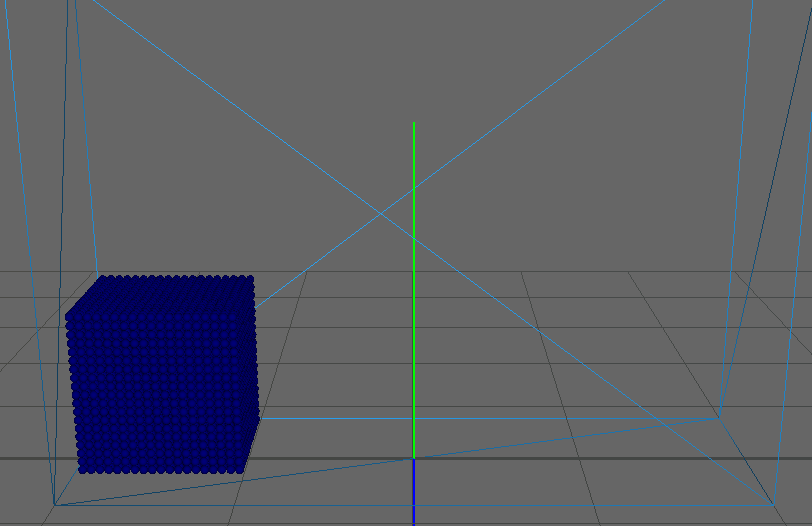
\includegraphics[width=\textwidth]{my-gfx/figure-dataset-1.png}  
    \end{subfigure}
    \hfill
    \begin{subfigure}[b]{0.475\textwidth}  
        \centering
        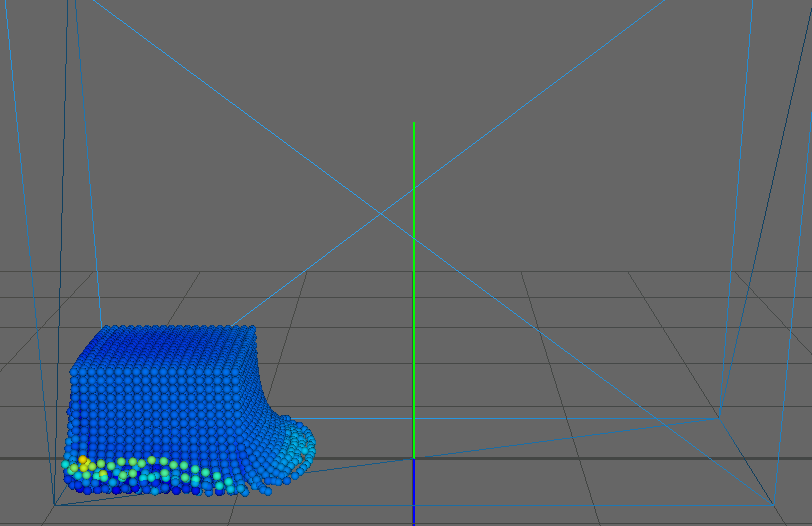
\includegraphics[width=\textwidth]{my-gfx/figure-dataset-2.png} 
    \end{subfigure}
    \vskip\baselineskip
    \begin{subfigure}[b]{0.475\textwidth}   
        \centering
        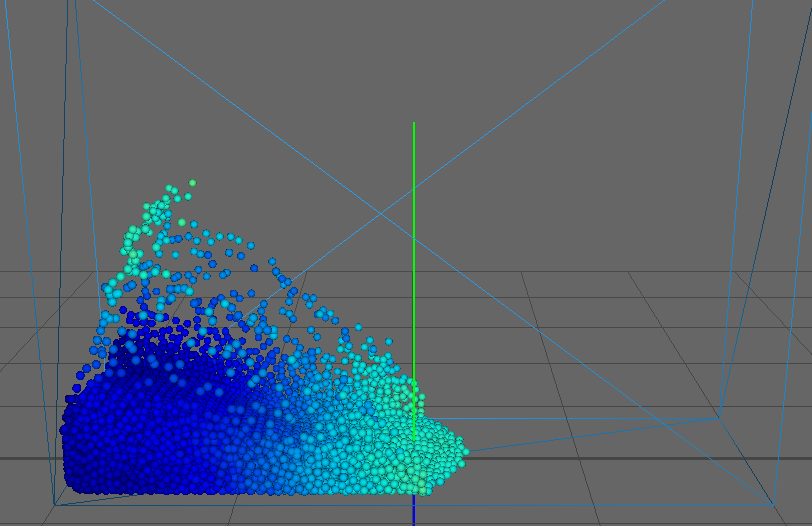
\includegraphics[width=\textwidth]{my-gfx/figure-dataset-3.png}  
    \end{subfigure}
    \hfill
    \begin{subfigure}[b]{0.475\textwidth}   
        \centering
        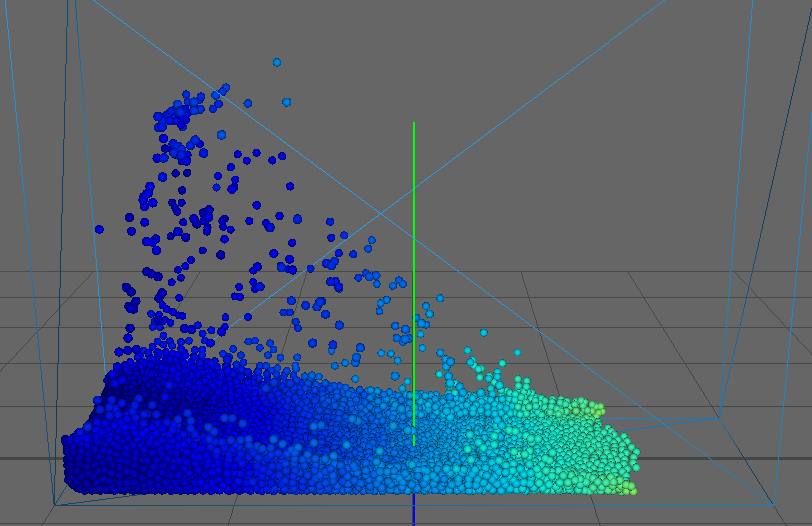
\includegraphics[width=\textwidth]{my-gfx/figure-dataset-4.png}
    \end{subfigure}
    
    \caption{Four simulation steps of our dataset: A cube of fluid dropping into a box (a so-called dam break scenario). Screenshots from the \textit{SPlisHSPlasH} application. The color gradient indicates the particles' velocity from low (blue) to high (green).}
    \label{fig:dataset}
\end{figure*}

As our main dataset for tests we used a typical dam break scenario, characterized by a block of fluid that drops into a confined box (Figure \myref{fig:dataset}). This frequently used dataset qualifies perfectly for our application as it features flat surfaces at the start (the block of fluid) and intricate edges and splashes as the block collides with the box, flinging into the air on the other side. We ran the simulation for about $10$ seconds, producing $123$ frames with $6859$ particles each.

%% !TEX root = ../my-thesis.tex
%
\chapter{Pipeline}
\label{sec:pipeline}

\section{Pipeline overview}
\label{sec:pipelineoverview}

\begin{figure}[htb]
	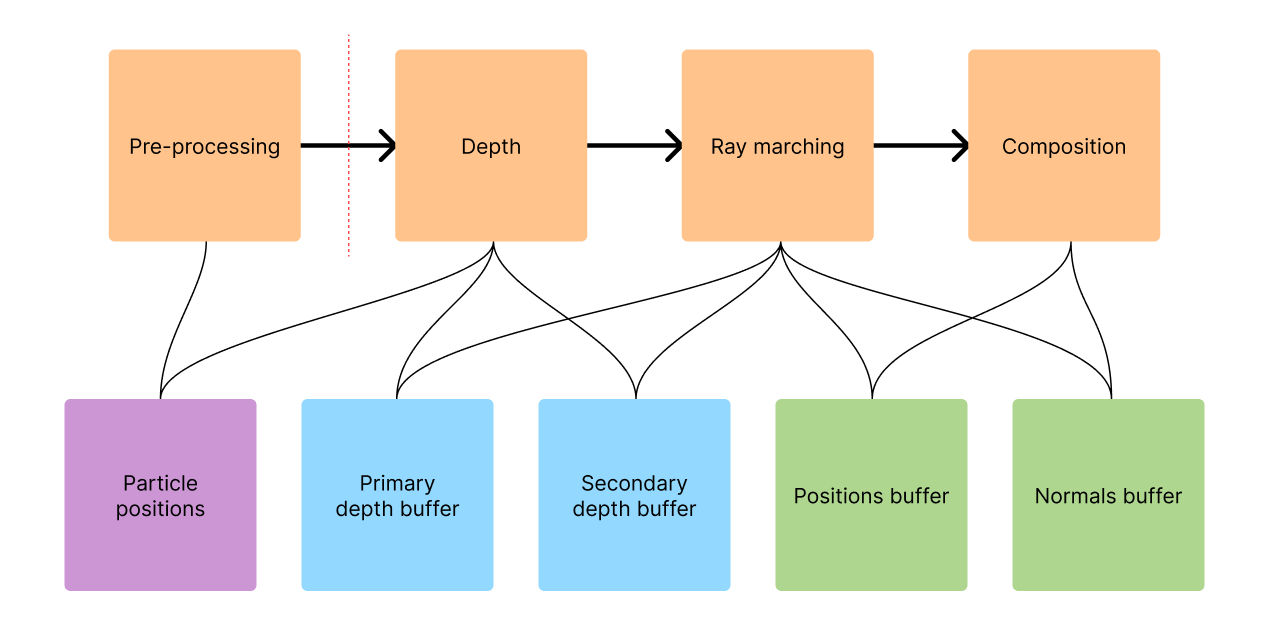
\includegraphics[width=\textwidth]{my-gfx/figure-pipeline.png}
	\caption{The computation pipeline and data flow of the program. The passes of the pipeline are displayed in orange. Regarding the data structures at the bottom: arrays are purple, depth buffers are blue, and color buffers are green. Pre-processing is decoupled in our implementation but can be incorporated into the per-frame computations.}
	\label{fig:pipelineoverview:pipeline}
\end{figure}

In this chapter, we show a high-level overview of the pipeline that all data flows through to eventually create an image on the screen. We aim to provide context for the following chapters that go more deeply into explaining the authors' work.

The proposed algorithm works through multiple passes, each one taking the output of the previous one as input. The input to the entire pipeline is an array of three-dimensional particle positions that represent the fluid at one particular moment in time. In Figure \myref{fig:pipelineoverview:pipeline}, we illustrate which part of the pipeline accesses which data structures.

\subsection{Pre-processing}

During this pass, the particle data is pre-processed and acceleration structures are built that serve the purpose of speeding up the following passes. An important note is that Wu et al. incorporate this pass into their algorithm tightly. It is executed in every frame of the visualization by processing it on the GPU. We on the other hand decided to run it only once when loading the dataset as it is the most time-consuming part of our implementation. We provide more information on how to improve on this in the chapter \textbf{Future work \myref{sec:futurework}}.

Firstly, the so-called \textit{binary density grid} (also called \textit{density mask} in the paper) is generated (Wu et al. \cite{Wu:2022}, section 4.1). Space is divided into a grid of cells. Each cell holds a boolean value indicating whether it is at all possible for the algorithm to find the fluid's surface inside the cell. For that, the maximum density of the fluid is approximated. If it does not exceed a certain threshold, the cell can safely be skipped to save valuable computation time.

Secondly, each particle is classified as either belonging to a dense ("\textit{aggregated}") or to a sparse part of the fluid (splashes). This information is used in the depth pass when deciding which depth buffer the particle should be rendered to (more in the chapter \textbf{Handling splash particles \myref{sec:splashparticles}}).

\subsection{Depth pass}

In the depth pass, particles are rendered to a depth buffer as spheres with the radius $h$. The positions on those spheres serve as good approximations of the true fluid surface. They are used as starting points for refinement during the ray marching pass.

Two depth buffers are filled during this pass. The authors call these $D$ and $D_{agg}$, we call them the primary and secondary depth buffer respectively. All particles are rendered to the primary buffer, but only the ones classified as "aggregated" are rendered to the secondary buffer. More information on this is provided in the sections \myref{sec:depth} and \myref{sec:splashparticles}.

\subsection{Ray marching pass}

Rays are shot from the camera into the scene along which the fluid surface is searched. The depth buffer from the previous pass is used to compute entry points for the rays (more in the chapter \textbf{Surface extraction with ray marching \myref{sec:surfaceextraction}}). Since this pass is very costly on its own,  the authors provide several adaptive techniques for reducing the time spent ray marching - for example a hash grid and variable resolution.

\subsection{Composition pass}

The last step of the pipeline is to take the data computed in all previous passes and determine a color for each pixel of the screen. Here, the fluid's properties like color, refraction, transparency, and light interaction are modelled and it is embedded into the scene (more in the chapter \textbf{Image composition \myref{sec:imagecomposition}}).

\section{Depth pass}
\label{sec:depth}

\begin{figure*}[h]
    \centering
    \begin{subfigure}[b]{0.475\textwidth}
        \centering
        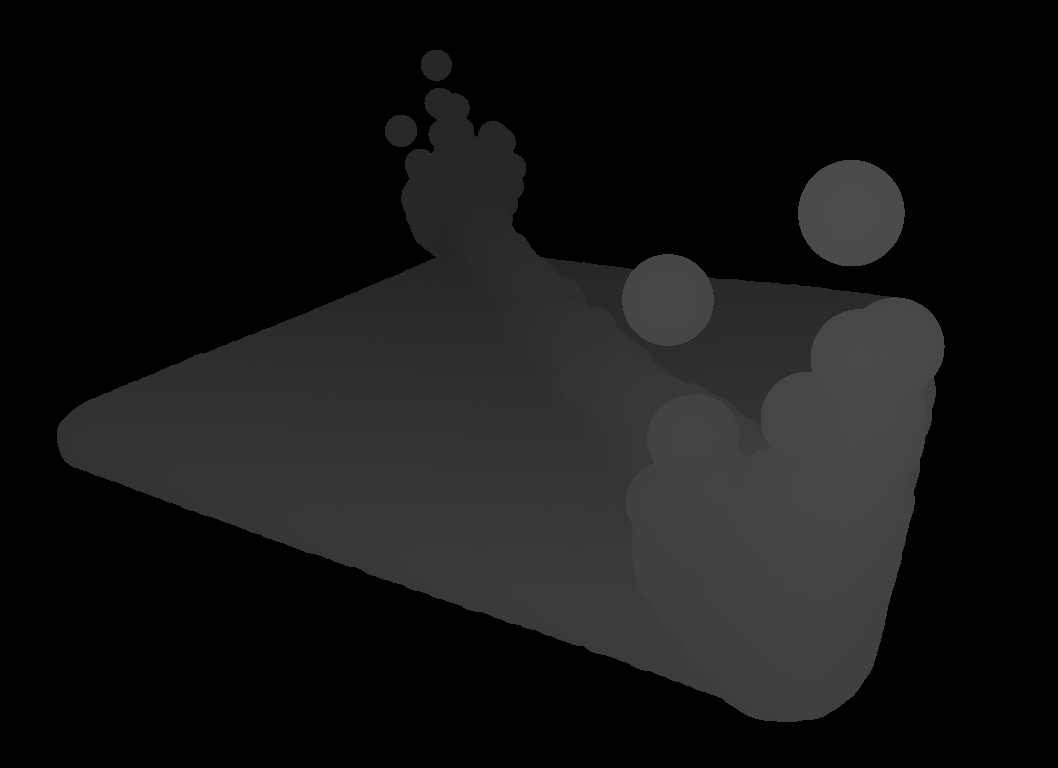
\includegraphics[width=\textwidth]{my-gfx/figure-depth-buffer-1.png}
    \end{subfigure}
    \hfill
    \begin{subfigure}[b]{0.475\textwidth}  
        \centering 
        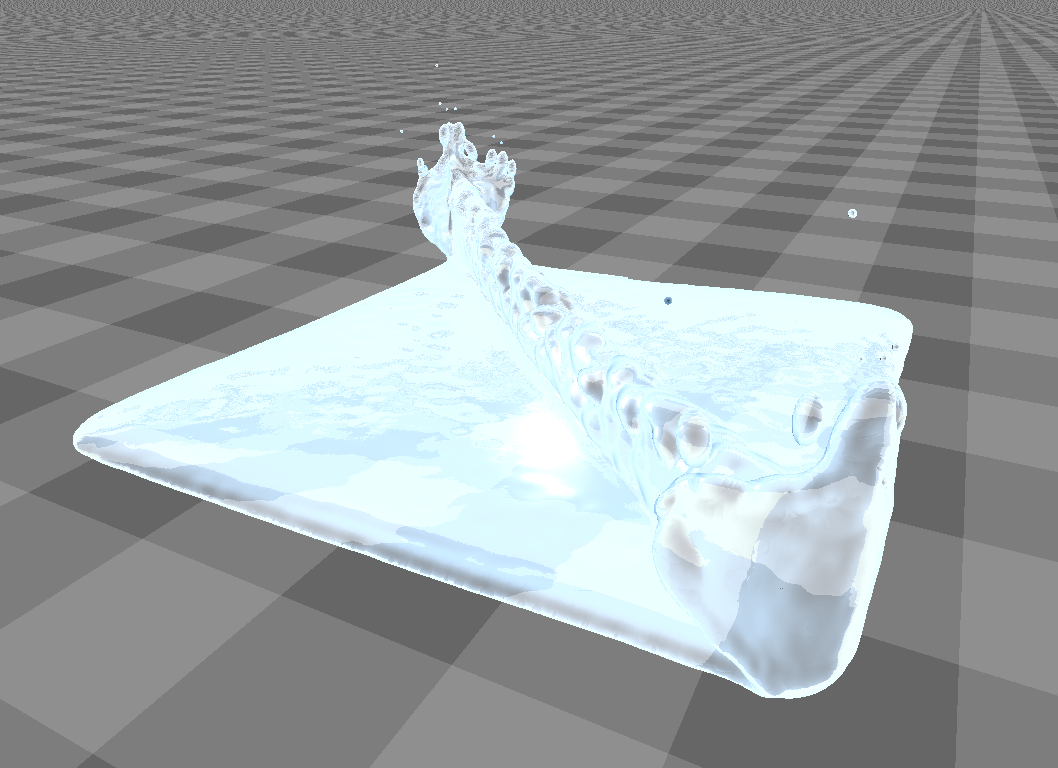
\includegraphics[width=\textwidth]{my-gfx/figure-depth-buffer-2.png}
    \end{subfigure}
    \vskip\baselineskip
    
    \caption{\textit{Left}: The depth buffer of a visualization frame (inverted). Particles appear as smooth spheres. Lighter areas are closer to the camera. \textit{Right}: The resulting image after the composition pass.}
    
    \label{fig:depthbuffer}
\end{figure*}

\begin{figure}[h]
    \centering
    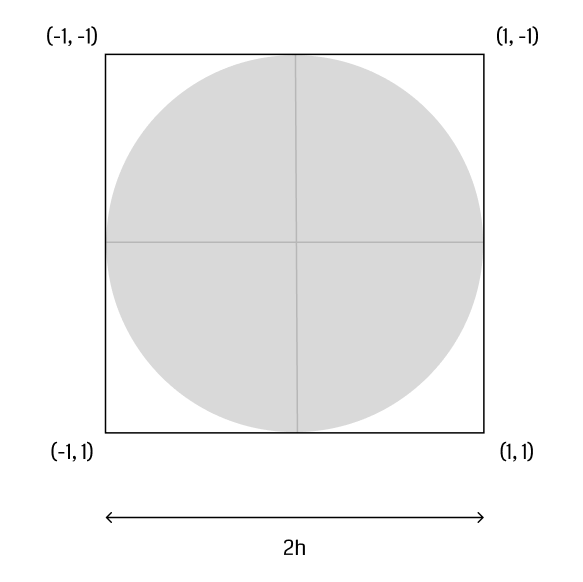
\includegraphics[width=0.5\textwidth]{my-gfx/figure-uvs.png}
    \caption{A quad of two triangles representing one particle. The texture coordinates are set up for computing a spherical offset in the z-direction}
    \label{fig:depth:uvs}
\end{figure}

After pre-processing has taken place, the particles are rendered into depth buffers that serve as entry points for the surface reconstruction (see Figure \myref{fig:depthbuffer} for a visualization of a depth buffer).

The first step is to construct a vertex buffer that holds all particles comprising the fluid. Wu et al. suggest to render a camera-facing quad for each particle with sidelength $2h$. Each vertex holds
\begin{enumerate}
    \item a three-dimensional position in world space,
    \item and a two-dimensional texture coordinate - $(-1, -1)$ for the top left, $(1, 1)$ for the bottom right vertex (Figure \myref{fig:depth:uvs}).
\end{enumerate}
The vertex buffer is fed into the first render pass, which writes to the depth buffers. The value output to the buffer is:
\[ depth := z - \cos(\frac{\pi}{2} r) \]
with $r := \sqrt{u^2 + v^2}$ being the world-space distance from the particle's center and $z$ being the particle's z-coordinate. The fragment is discarded if $r > 1$.

This technique renders the particles as if they were perfect spheres - although they are rendered simply as two triangles - by projecting onto the surface of the camera-facing hemispheres surrounding the particles. Conveniently, by using a depth buffer for this pass, occlusion is handled efficiently by the graphics hardware.

Two depth buffers will be filled using this technique:
\begin{enumerate}
    \item the \textit{primary} depth buffer (called $D$ in the paper) containing all particles
    \item and the \textit{secondary} depth buffer (called $D_{agg}$ in the paper) containing only particles belonging to a denser ("aggregated") part of the fluid volume.
\end{enumerate}
The former will be used as a first estimation of the fluid's surface. The latter will be used to enable the ray marcher to skip large parts of empty space and continue at the surface again (further details in chapter \textbf{Methods of acceleration \myref{sec:acceleration}}).


\section{Surface extraction with ray marching}
\label{sec:surfaceextraction}

Ray marching has gained popularity in recent years as a surface extraction method for particle-based representations as it suits the parallel nature of computation on GPUs. It can be implemented in a compute or fragment shader and executed independently. Although this is the way the authors designed their implementation, we had to refrain from following that path for lack of time. This step, however, would lead to significant reductions in computation time.

Ray marching refers to a technique of sampling some function at points along a ray and collecting information about the function in the process. In our application, we shoot rays from the camera to sample the fluid's density $\rho$ and find a point where the surface criterion is met (see the surface definition \myref{sec:surfacedefinition}). Theoretically - since the fluid is continuous -, infinitely many rays would be needed to capture the entire surface. For graphical applications, however, the finest granularity of information can be retrieved at the pixel level. Any surface information between pixels would not - at least not in the algorithm discussed here - contribute to the final image. Hence, all the following computations are performed for each pixel of the screen (of size $WIDTH \times HEIGHT$) labeled $i$.

In mathematical terms, we search for a point $\textbf{r}$ along the ray
\[ \textbf{r} = \textbf{a} + t \textbf{v}, \space t \in [0, \infty) \]
where the following condition is satisfied:
\[ \rho ( \textbf{r} ) = \sigma. \]
In the ray equation, $\textbf{a}$ is the starting position of the ray and $\textbf{v}$ is a unit-vector indicating the direction the ray is travelling in. They can be computed by applying the inverse transformation pipeline ($\textbf{P}$ being the projection and $\textbf{V}$ being the camera matrix) to the homogenous clip space coordinates $( x, y, z, 1 )^T$:
\[
\tilde{\textbf{a}} :=
\begin{pmatrix}
\tilde{\textbf{a}}_x \\
\tilde{\textbf{a}}_y \\
\tilde{\textbf{a}}_z \\
\tilde{\textbf{a}}_w
\end{pmatrix} =
\textbf{V}^{-1} \space \textbf{P}^{-1} \space
\begin{pmatrix} x \\ y \\ z \\ 1 \end{pmatrix}
\]
$z \in [0, 1]$ is looked up directly from the primary depth buffer. If $z = 1$, the depth pass did not output a value for this pixel, meaning there is no fluid surface to be found. In this case, the pixel can be discarded. $x, y \in [-1, 1]$ are retrieved with the following computations. The pixel coordinates are converted to so-called normalized device coordinates:
\[ x := 2 \frac{i \text{ mod } WIDTH + 0.5}{WIDTH} - 1 \]
\[ y := 2 \frac{\lfloor i / WIDTH \rfloor + 0.5}{HEIGHT} - 1 \]
where $i$ is the index of the current pixel counting row-wise from the origin of the screen. The origin depends on the used graphics API (\textit{OpenGL} handles this differently than \textit{Vulkan}, for example).

Since we are dealing with homogenous coordinates in projective space, $\tilde{\textbf{a}}$ needs to be dehomogenized to be used as a three-dimensional coordinate:
\[
\textbf{a} := \frac{1}{\tilde{\textbf{a}}_w}
\begin{pmatrix}
\tilde{\textbf{a}}_x \\
\tilde{\textbf{a}}_y \\
\tilde{\textbf{a}}_z
\end{pmatrix}
\]
To obtain the ray's direction, we must only compute a vector pointing from the camera's position $\textbf{c}$ to the start of the ray $\textbf{a}$ and normalize it:
$$\textbf{v} := || \textbf{a} - \textbf{c} ||$$
Now we have defined a viewing ray with an entry point right near the fluid's surface which greatly decreases the number of ray marching steps needed to find the iso-surface.

\subsection{Marching along the ray}

When stepping forward on the ray, it is common to increment $t$ (of the ray equation) in uniform steps at the start of each iteration. However, as the number of necessary steps is the limiting factor for performance in all ray marching algorithms, it is desirable to omit unnecessary steps wherever possible. Such optimizations are described further below. For now, we assume that in each iteration, $\textbf{r}$ will be moved forward by equal step sizes $\Delta t$:
\[ \textbf{r}' := \textbf{r} + \Delta t \textbf{v}. \]
The step size should be set as a fraction of the particle radius $h$ so no particles are skipped. The first time we encounter a position where $\rho(\textbf{r}) \geq \sigma$ - we cannot check for exact equality when moving in discrete steps - the surface's position is assumed there. The position can then be stored in a buffer holding a three-dimensional position for every pixel of the screen. When we find the surface's position, we also want to compute the normal for lighting calculations during image composition. For this, the authors propose to sum up the gradients of the kernel function (see equation 11 of Wu et al. \cite{Wu:2022}):
\[
\textbf{n}_{object}(\textbf{r}) = || \space \sum_i \nabla W(\textbf{r}_i - \textbf{r}) \space ||
\]
The gradient is a vector pointing radially outward from the particle's position $\textbf{r}_i$ to the evaluation point $\textbf{r}$. Summing these up essentially averages over all particle's normals - weighted by the kernel function - creating a representative normal vector for the fluid surface.

\subsection{Implementation}

The way we implemented the ray marching is via a pool of CPU threads that is always ready to do work. When the threads are signalled, they go through each pixel of the screen and evaluate the surface parameters in the direction of the pixel. This drastically improves performance over the sequential algorithm with a theoretical speedup equal to the number of threads used because there is no need for inter-thread communication. As mentioned above, by employing the massive parallelism of graphics hardware, one can achieve much better results.

The underlying data structures are simple floating-point image buffers with sizes equal to the screen:
\begin{enumerate}
    \item the \textit{depth buffers} used for determining each ray's starting point,
    \item a \textit{color buffer} for the fluid surface's position per pixel,
    \item and a \textit{color buffer} for the fluid surface's normal per pixel.
\end{enumerate}


\section{Image composition}
\label{sec:imagecomposition}

In this last step of the pipeline, the computed per-pixel fluid properties are used to construct an image that will be presented on the screen. The authors did not state specifics about this phase of the algorithm, so this chapter can be viewed as an explanation of our implementation.

For each pixel, we compute
\begin{enumerate}
    \item a diffuse color,
    \item a specular color using Phong's lighting model (Phong \cite{Phong:1975}),
    \item an environment color from reflection or refraction
\end{enumerate}
and combine these to form the resulting pixel color.

The fluid's physical properties are incorporated into the computation of these colors like shininess, refraction index, opacity, and apparent color.

\subsection{Normals}

The authors propose a technique they call \textit{adaptively blended normals}. The idea is to interpolate between two normal vectors depending on the distance of the camera to the fluid surface. One of those normals $\textbf{n}_{object}$ comes from the summation of the kernel's gradient - as described in the previous section. The second one is a screen-space normal $\textbf{n}_{screen}$ that is extracted from a smoothed version of the primary depth buffer $D$. The smoothing is a Gaussian blur that can be efficiently computed on the GPU.

This blending of normals aims to reduce the spherical features that are present in the depth buffer. Even after filtering, the particles' spherical shape cannot be hidden sufficiently when they appear big on screen - i. e. the camera is close to the fluid. Therefore, Wu et al. suggest to use $\textbf{n}_{object}$ to correct the screen space normal.

\subsection{Implementation}

We implemented this pass in a fragment shader that runs on the GPU. A triangle that spans the entire screen is rendered so that the GPU evaluates the shader for every pixel.

The following data structures are available to the composition pass:
\begin{enumerate}
    \item a world-space position of the surface for each pixel
    \item and a world-space normal of the surface for each pixel.
\end{enumerate}
They are accessed through texture samples from the shader, using the pixel's position as texture coordinates.

Our environment consists of a floor texture that is generated right inside the shader using a combination of step and modulo functions. This way, the refractions of the fluid are made visible. Usually, an environment map of the surrounding scene would be generated that can be sampled to let the fluid reflect and refract light from the scene.

Although we did not implement the screen-space normal extraction and blending, we found the object normals to be an excellent approximation for achieving realistic lighting. However, we would like to implement this in the future to see the effect and evaluate if it significantly enhances the visualization quality.

%% !TEX root = ../my-thesis.tex
%
\chapter{Particle neighborhood and anisotropic kernels}
\label{sec:particleneighborhood}

\section{From isotropic to anisotropic}

We explained the smoothing kernels used in \textbf{Smoothed Particle Hydrodynamics \myref{sec:sph}} above and called them isotropic - which can be thought of as "spherical" or radially homogenous. This property is necessary for simulation but leads to the most prominent visual artifacts of visualizing particle-based surfaces: Flat surfaces no longer look flat but rather bumpy. It can be evidently seen that the underlying representation is made up of points or spheres. The authors compared their method to multiple others, illustrating the need for a way of hiding spherical artifacts (see Figure 8 of Wu et al. \cite{Wu:2022}). To combat this, researchers have begun to develop anisotropic techniques for the extraction of surfaces from point clouds as soon as 2001 (Dinh et al. \cite{Dinh:2001}).

Interestingly, the main idea has not changed over the last 20 years seeing that Wu et al. use a very similar technique as described in that 2001 paper:
For a given point in space, the configuration of the neighboring points is characterized with a principal component analysis to retrieve the main axes along which the particles are distributed. This information is used to stretch the surface in a way that better fits the particles' distribution. This has the effect of preserving sharp features like edges and corners as well as flat, homogenous areas.

In our case, "stretching the surface" means transforming the input vector to the kernel function with a linear transformation matrix $\textbf{G}$ consisting of rotation and non-uniform scaling (further information below in \textbf{Particle classification \myref{sec:particleclassification}}):
\[
W_{a} ( \textbf{r}, \textbf{G} ) :=
c \space \det (\textbf{G}) \space P ( | \textbf{G} \textbf{r} | )
\]
Comparing to the isotropic kernel function $W$, the authors substitute $\frac{1}{h^3}$ for the determinant of $\textbf{G}$ and apply the linear transformation to the input of $P$.
This kernel can be reduced to the isotropic kernel by setting $\textbf{G} := h^{-1} \textbf{I}$ where $\textbf{I}$ is the three-dimensional identity matrix.

\section{Neighborhood definition}

The neighborhood $N$ of a point $\textbf{r}$ is defined as the set of the indices of all particles that lie in a sphere with radius $R_N$ around that point:
$$N (\textbf{r}, R_N) := \{ i \in \{ 0,...,n-1 \} : | \textbf{r}_i - \textbf{r} | < R_N \}$$

\section{Neighborhood search}

The authors did not mention the algorithm they used to find neighboring particles. The de facto standard spatial acceleration structure for SPH-related algorithms is the hash grid. For this reason, we opted to incorporate this approach as well, leaning on the explanation by Koschier et al. \cite{Koschier:2019}. A hash grid divides space into equally sized cells. A cell index can then be computed for an arbitrary point $\textbf{r}$ by dividing by the cell size $c$ and rounding each entry down to the closest integer:
\[
\begin{pmatrix} i \\ j \\ k \end{pmatrix} :=
\lfloor c^{-1} \space \textbf{r} \rfloor =
\begin{pmatrix}
\lfloor c^{-1} \space x \rfloor \\
\lfloor c^{-1} \space y \rfloor \\
\lfloor c^{-1} \space z \rfloor \\
\end{pmatrix}
\]
The cell index can then be hashed using any function $hash: \mathbb{Z}^3 \rightarrow \mathbb{Z}$ to retrieve an index into a table storing some data associated with the cell. In this case, we store a list of indices of particles lying in the cell.

We use a library called \textit{CompactNSearch} developed by Dan Koschier \cite{CompactNSearch} which is also used by the \textit{SPlisHSPlasH} framework \cite{SplishSplash} we use for dataset generation. It uses the technique described above to accelerate neighborhood search in a point cloud for a given neighborhood radius which is equal to the cell size $c := R_N$. The hashing function is efficient, consisting only of simple prime number multiplications (using prime numbers $p_0,p_1,p_2$) and XOR operations ($\otimes$):
\[
hash(i,j,k) :=
p_0 i \otimes
p_1 j \otimes
p_2 k
\]
Koschier keeps their implementation straightforward by using the C++ standard library's \textit{std::unordered\_map} as a hash table, providing the custom hash function mentioned above.

Each value of the hash table holds an array of integers representing the indices of the particles contained in the cell.

So, when querying the neighbors of a point $\textbf{r}$, every particle in the $3 \times 3 \times 3$ neighborhood of that cell has to be tested for inclusion. This is because the cells' width is equal to the search radius. The test looks as follows:
\[ |\textbf{r}_i - \textbf{r}| < R_N \]
or more efficiently as calculating a root is slower than multiplication:
\[ (\textbf{r}_i - \textbf{r})^2 < R_N^2 \]
We use two separate search grids:
\begin{enumerate}
    \item one for density calculation - for which we set $R_N := h$ -
    \item and one for anisotropy calculation - for which we set $R_N := 2h$.
\end{enumerate}

The first one is used whenever we compute $\rho(\textbf{r})$. Using the kernel's property of having finite support - meaning $W(\textbf{r}) = 0$ for $|\textbf{r}| \geq h$ -, the summation does not have to iterate over all particles of the system. Instead, we perform a neighborhood search to greatly reduce the number of operations necessary to calculate the density.

The second search grid is used for characterizing the neighborhood of each particle $i$ to obtain a transformation $\textbf{G}_i$. It is used in the anisotropic kernel function when computing $\rho$.

A naive loop over all $n$ particles means the evaluation of $\rho$ has a lower bound of $\mathcal{O}(n)$. Because accessing the hash table is a constant-time operation, spatial hashing reduces the time complexity to approximately $\mathcal{O}(\overline{|N|})$ where $\overline{|N|}$ is the expected number of neighbors.

It is also important to consider how cells are ordered in memory. Modern hardware implements extensive caching capabilities that are essential for performant software. Programmers are advised to keep memory locations that are accessed together close to each other. Since for every neighborhood search, 27 cells have to be looked up, it is beneficial to store these 27 cells as close to each other as possible. Koschier therefore sorts the grid in a z-curve arrangement, allowing for spatial coherence when arranging a three-dimensional grid in a one-dimensional array (see Figure \myref{fig:z-curve} for a two-dimensional illustration).

\begin{figure}[htb]
    \centering
    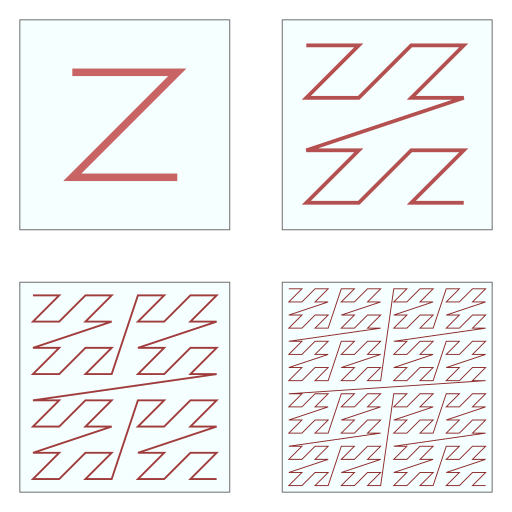
\includegraphics[width=0.75\textwidth]{my-gfx/figure-z-curve.png}
    \caption{A z-curve ordering of two-dimensional grids of varying sizes. The image comes from the public Wikimedia Commons repository \cite{ZCurve}.}
    \label{fig:z-curve}
\end{figure}


\section{Weighted Principal Component Analysis}

Principal component analysis is a common method of reducing the dimensionality of datasets to enable visualization in two or three dimensions (Koren et al. \cite{Koren:2003}). This is achieved by finding orthogonal axes that best fit the data and project it onto a subset of those axes. Since we are not dealing with high-dimensional data, we are not interested in reducing its complexity. Rather, we want to find the axes that most closely match the configuration of points in a small neighborhood. To do this, one has to compute the eigenvectors of the correlation matrix derived from the point set.

In this section, we explain the algorithm Wu et al. use to compute the principal components. It depends on the work of Yu and Turk \cite{Yu:2013} where an alteration of standard PCA is employed called Weighted Principal Component Analysis (WPCA). The key difference is that each point $\textbf{r}_j$ is assigned a weight $w_{j} \in \mathbb{R}$ that is used when computing the dataset's correlation matrix $\textbf{C}$ and mean $\overline{\textbf{r}}$.

We define the correlation matrix as not limited to evaluation at the particles' positions. This differs from our sources (Yu and Turk \cite{Yu:2013}) in that we can characterize the neighborhood around any point in space. The reason for this is explained below in \textbf{Implementation \myref{sec:particleneighborhood:implementation}}.
\[
\textbf{C}(\textbf{r}) :=
\frac{1}{\sum_j w_{j}}
\sum_j w_j (\textbf{r}_j - \overline{\textbf{r}}) (\textbf{r}_j - \overline{\textbf{r}})^T
\]

\[
\overline{\textbf{r}} :=
\frac{1}{\sum_j w_j}
\sum_j w_j \textbf{r}_j
\]
For weights, some isotropic smoothing kernel $W$ is used. We use the one described in \textbf{Smoothed Particle Hydrodynamics \myref{sec:sph}}:
\[ w_j := W(\textbf{r}_j - \textbf{r}) \]
Applying weights to the particles' positions can be interpreted as an analogy to the SPH method. It also reduces visual artifacts because there is no strict boundary between lying inside and outside the neighborhood of a point.

After computing $\textbf{C}$, an eigendecomposition is performed on this matrix. The matrix is decomposed into a rotation $\textbf{R}$ and a scaling $\bm{\Sigma}$ containing $\textbf{C}$'s eigenvalues on its diagonal (see equation 12 in Yu and Turk \cite{Yu:2013}):
\[ \textbf{C} = \textbf{R} \bm{\Sigma} \textbf{R}^T \]

\section{Singular neighborhood configurations}

Some neighborhood configurations might yield a correlation matrix whose determinant is close or equal to zero. This can happen when all points lie on the same plane. In this case, the eigendecomposition returns a small eigenvalue leading to exploding numbers when computing $\bm{\Sigma}^{-1}$. To address this problem, Yu and Turk introduce a minimum for each eigenvalue as a fraction of the largest one. This way, the deformation can be controlled and parameterized to fit different use-cases.

Assuming $\sigma_1 \geq \sigma_2 \geq \sigma_3$, a new $\tilde{\bm{\Sigma}}$ is constructed with the altered eigenvalues, limiting the ratio of two eigenvalues to a constant $k_r$ (see equation 15 in Yu and Turk \cite{Yu:2013}):
\[ \tilde{\sigma}_k := \max \{ \sigma_k, \frac{\sigma_1}{k_r} \} \]
\[
\tilde{\bm{\Sigma}} :=
\begin{cases}
k_s \text{diag}(\tilde{\sigma}_1, \tilde{\sigma}_2, \tilde{\sigma}_3) & |N| > N_{\epsilon}, \\
k_n \textbf{I} & else
\end{cases}
\]
\[ \tilde{\textbf{C}} := \textbf{R} \tilde{\bm{\Sigma}}^{-1} \textbf{R}^T \]

We define $\tilde{\textbf{C}}(\textbf{r})$ as a function that computes $\textbf{C}(\textbf{r})$ as above and alters it, returning $\tilde{\textbf{C}}$.

The parameters of this algorithm are explained briefly. Note that they are dataset-dependent and the provided values work well with our dataset.
\begin{enumerate}
    \item $k_r \geq 1$ limits the maximum deformation relative to the largest eigenvalue. Large values lead to large deformations. We used $k_r := 2$.
    \item $k_s$ merely scales all eigenvalues. We used $k_s:= 2000$.
    \item $N_{\epsilon}$ is a threshold for the number of neighbors $|N|$. The deformation is not applied for really small neighborhoods. In this case, particles are displayed as spheres whose radius can be adjusted with $k_n$. This will prevent spray particles with few neighbors to be displayed as big ellipsoids. We set $N_{\epsilon} := 15$ and $k_n := 1$.
\end{enumerate}

In the following, the altered covariance matrix $\tilde{\textbf{C}}$ will be used to retrieve a transformation from isotropic to anisotropic space.

\section{Particle classification}
\label{sec:particleclassification}

\begin{figure}[htb]
	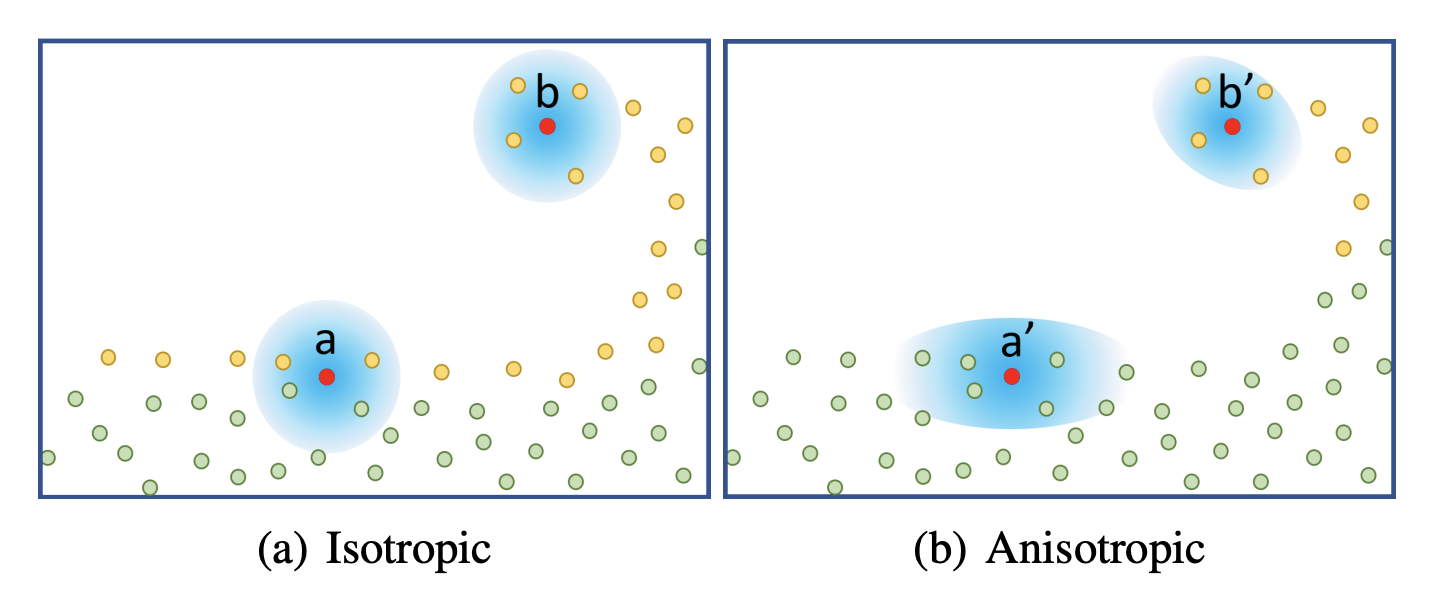
\includegraphics[width=\textwidth]{my-gfx/figure-anisotropic.png}
	\caption{This is figure 4 of the paper by Wu et al. \cite{Wu:2022}. It shows how anisotropic kernels help with correctly classifying particles located close to the surface of the fluid.}
	\label{fig:particleneighborhood:anisotropic}
\end{figure}

In order to reduce the number of ray marching steps near small bundles of particles, they have to be classified as either belonging to a dense fluid area ("aggregated") or to a sparse area (non-aggregated, splash particles). For this, the density is evaluated at each particle's position and compared to a constant. When using isotropic kernels for the density calculation, this will lead to misinterpretations at the surface of the fluid, even in aggregated locations (Figure \myref{fig:particleneighborhood:anisotropic}). Therefore, the authors suggest to characterize the particle's neighborhood as explained above and construct a transformation matrix $\textbf{G}_i$ for the particle to be used as an input to the anisotropic kernel $W_a$. $\textbf{G}_i$ is a transformation into the coordinate system represented by $\tilde{\textbf{C}}$, so it has to be the inverse of $\tilde{\textbf{C}}$ (note that $\textbf{R}$ is a rotation matrix, therefore $\textbf{R}^{-1} \equiv \textbf{R}^T$):
\[
\textbf{G}_i :=
h^{-1} \tilde{\textbf{C}}_i^{-1} =
h^{-1} (\textbf{R} \tilde{\bm{\Sigma}} \textbf{R}^T)^{-1} =
h^{-1} \textbf{R}^{-T} \tilde{\bm{\Sigma}}^{-1} \textbf{R}^{-1} =
h^{-1} \textbf{R} \tilde{\bm{\Sigma}}^{-1} \textbf{R}^T
\]
where $\tilde{\textbf{C}}_i := \tilde{\textbf{C}}(\textbf{r}_i)$ is the altered correlation matrix from above evaluated at the particle's position $\textbf{r}_i$.

Now, to compute the density at $\textbf{r}$, we use the anisotropic kernel function and only take those particles into consideration which are in the neighborhood $N$ of $\textbf{r}$:
\[
\rho(\textbf{r}) = m \sum_{i \in N(\textbf{r}, h)} W_a(\textbf{r}_i - \textbf{r}, \textbf{G}_i)
\]

This leads to a significant improvement in image quality as can be seen in Figure \myref{fig:anisotropy}.

\begin{figure*}
    \centering
    \begin{subfigure}[b]{0.475\textwidth}
        \centering
        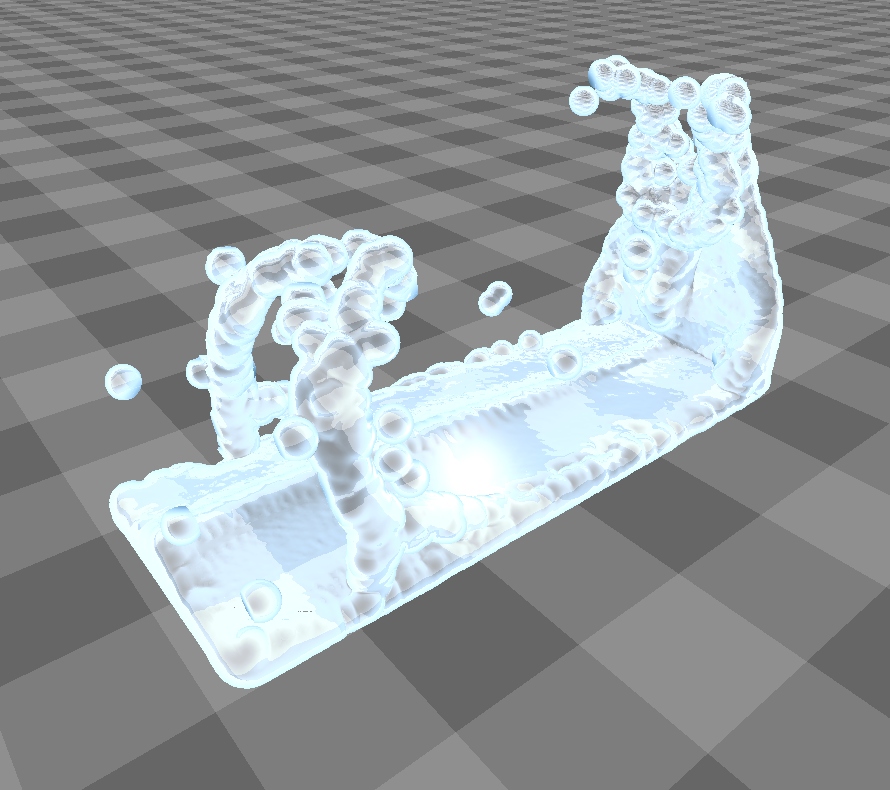
\includegraphics[width=\textwidth]{my-gfx/figure-anisotropy-1.png}  
    \end{subfigure}
    \hfill
    \begin{subfigure}[b]{0.475\textwidth}  
        \centering 
        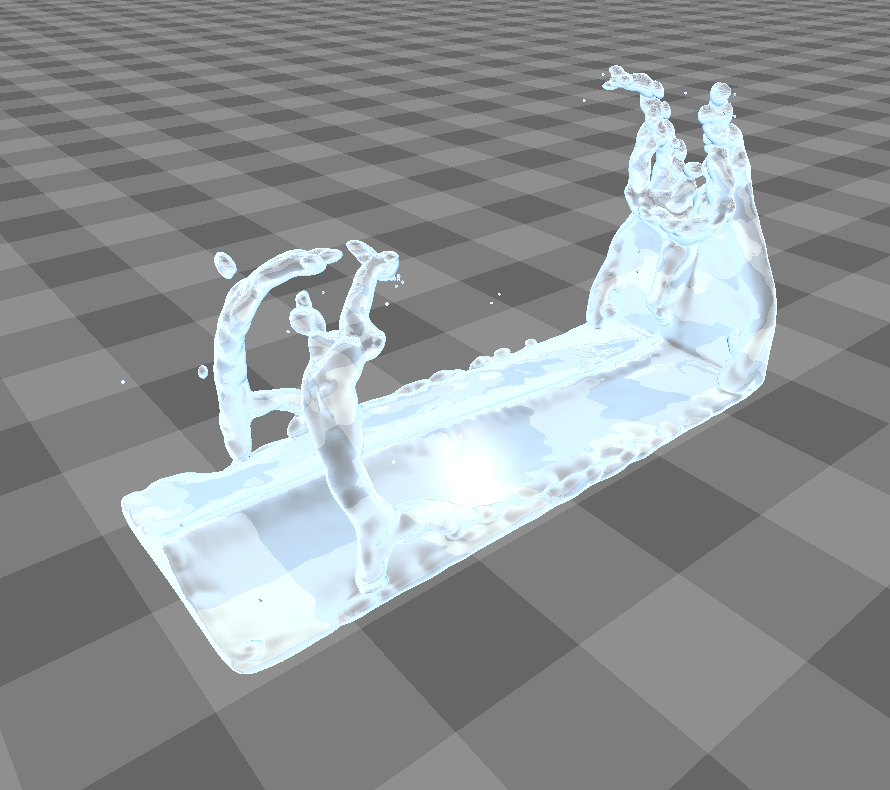
\includegraphics[width=\textwidth]{my-gfx/figure-anisotropy-2.png} 
    \end{subfigure}
    \vskip\baselineskip
    
    \caption{\textit{Left}: A visualization frame with isotropic kernels. Particles appear spherical and homogenous. \textit{Right}: The same scene with anisotropic kernels. The deformation is dependent on the neighborhood of each particle, creating a more interesting picture.}
    \label{fig:anisotropy}
\end{figure*}


\section{Implementation}
\label{sec:particleneighborhood:implementation}

Because the correlation matrix $\textbf{C}$ representing a neighborhood configuration is symmetric (see the following equation) and real and therefore self-adjoint - meaning $\textbf{C} = \overline{\textbf{C}^T}$ and specifically $\overline{\textbf{C}^T} = \textbf{C}^T$ for real matrices -, an algorithm called \mbox{\textit{SelfAdjointEigenSolver}} of the \textit{Eigen} library can be employed.
In the following equation, the brackets are used to differentiate indices from one another. We use $[\textbf{C}_i]_{mn}$ to refer to the element in the $m$-th row and $n$-th column of matrix $\textbf{C}_i$. Likewise, $[\textbf{x}_i]_n$ refers to the $n$-th entry of the vector $\textbf{x}_i$.
\[
\textbf{C}(\textbf{r}) :=
\frac{1}{\sum_j w_{j}}
\sum_j w_j (\textbf{r}_j - \overline{\textbf{r}}) (\textbf{r}_j - \overline{\textbf{r}})^T
\Rightarrow
\]
For $n,m = 1, 2, 3$:
\begin{align*}
[\textbf{C}(\textbf{r})]_{mn} &=
\frac{1}{\sum_j w_j} \sum_j w_j \space [\textbf{r}_j - \overline{\textbf{r}}]_m \space [\textbf{r}_j - \overline{\textbf{r}}]_n
\\ &=
\frac{1}{\sum_j w_j} \sum_j w_j \space [\textbf{r}_j - \overline{\textbf{r}}]_n \space [\textbf{r}_j - \overline{\textbf{r}}]_m
\\ &=
[\textbf{C}(\textbf{r})]_{nm}
,
\end{align*}

of which follows that $\textbf{C} = \textbf{C}^T$. This is also apparent because the outer product $\textbf{x} \textbf{x}^T$ itself is symmetric.

\textit{Eigen} uses a direct computation of eigenvalues and -vectors for three-by-three matrices by solving the equation $\textbf{A} \textbf{x} = \lambda \textbf{x}$ for the self-adjoint matrix $\textbf{A}$. There are iterative algorithms to achieve more accurate results but for the sake of performance, we chose to use the direct method.

Note that some math libraries automatically sort the computed eigenvectors by their associated eigenvalues in descending order. Others do not to reduce performance overhead when sorting is not needed. \textit{Eigen} belongs to the latter category. We could not rely on the eigenvalues being sorted, which was one source of errors during development.

\textbf{Note } At first, we performed the PCA at every step of the ray marching process. This led to greater visual fidelity as the granularity of the neighborhood determination was not restricted to the particle positions. But pre-computing the PCA for every particle up front - as Wu et. al suggest and as elaborated above - and using the resulting neighborhood matrix $\textbf{G}_i$ during ray marching is significantly faster while still bringing the advantages of anisotropic kernels. It could however be possible to perform the characterization during ray marching by fully porting the program to the GPU. Evaluations concerning this will have to be made in the future.

When finding the neighboring particles using the hash grid for neighborhood characterization, we use a search radius of twice the particles' radius: $R_N := 2h$. We found this to be a good compromise between over- and underfitting of the principal axes.

\section{Recap}

We have now introduced the transition from isotropic to anisotropic kernel functions and its necessity for high-quality surface reconstruction. We will now discuss the need for classification of particles into two groups. Furthermore, the key propositions of our primary source will be introduced and its effects will be evaluated.

%% !TEX root = ../my-thesis.tex
%
\chapter{Methods of acceleration}
\label{sec:acceleration}

Up until this chapter, most aspects of the algorithm we discussed build on papers that Wu et al. used as a basis during their research. Next, we introduce the main propositions they developed, which all contribute to making the algorithm faster and viable for real-time application. In order to accomplish this, the execution time of the algorithm has to be below $16.\overline{6}\text{ms}$ to be running at $60$ frames per second.

\section{Handling splash particles}
\label{sec:splashparticles}

\begin{figure}[h]
    \centering
    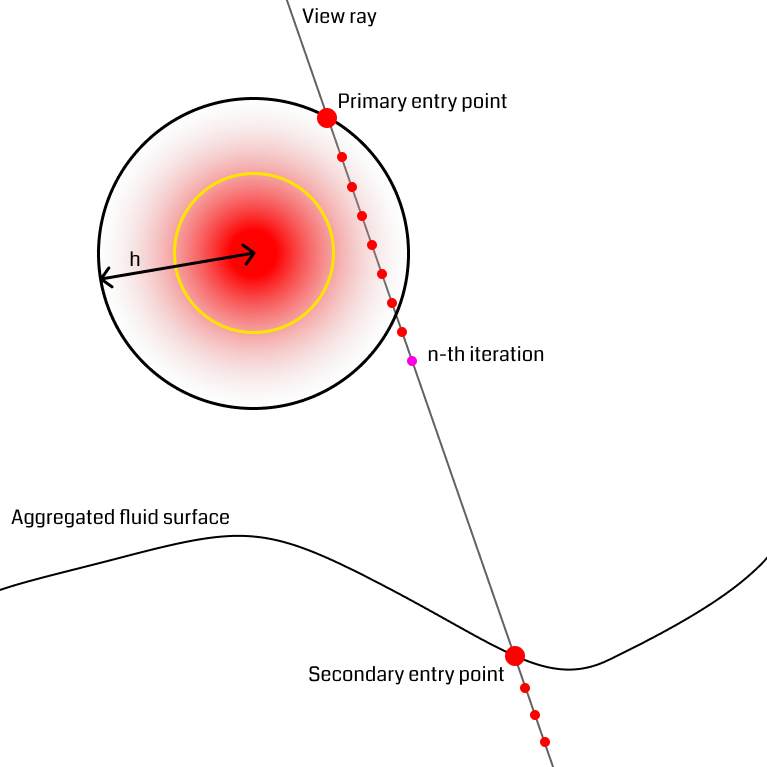
\includegraphics[width=0.75\textwidth]{my-gfx/figure-splash.png}
    \caption{The ray marching starts at the point extracted from the primary depth buffer. Here, the ray does not reach $\sigma$ (the iso-surface, indicated in yellow) in $n$ iterations. It can now skip to the point extracted from the secondary depth buffer which only aggregated particles were rendered to. The red gradient represents the kernel function of a particle.}
    \label{fig:splash}
\end{figure}

It is often the case that small bundles of particles fly up above the denser part of the fluid (Figure \myref{fig:splash}). Consider the rays starting at the outer rim of the splash particle's sphere. When traversing through the outer part of the sphere, they are unlikely to reach the density threshold $\sigma$ before exiting the sphere at the backside. In this situation, the ray would have to take a lot of steps to reach the next part of the fluid. The solution the authors suggest uses the previously mentioned secondary depth buffer $D_{agg}$ that only particles whose density exceeds a certain threshold are rendered to, omitting low-density areas like splash particles. When a ray reaches a certain number of steps and has not found an iso-surface yet, it computes a new position from the secondary depth buffer and continues from there, effectively skipping empty space and restarting near the fluid surface. This technique once more has the effect of reducing the number of ray marching steps.

\section{Adaptive step lengths}

The authors propose a data structure that helps reduce the number of steps during ray marching they call \textit{binary density grid} or \textit{density mask}. This enables the ray marcher to adapt the length of steps on the ray depending on the fluid's density in the surrounding area. To achieve this, a grid of cells is generated holding a boolean value indicating whether or not a surface can be expected in this cell.

Equation 1 of the paper states this criterion for every cell $c$:
\[
M_c := \begin{cases}
1 & \rho_c^{max} \geq \sigma, \\
0 & else
\end{cases}
\]
It is now the goal to determine an approximation of the maximum possible density $\rho_c^{max}$ inside the cell.

For every point $\textbf{r}_c$ inside cell $c$, we have (see equation 3 in \cite{Wu:2022})
\[
\rho(\textbf{r}_c) =
m \sum_{i \in N(\textbf{r}_c, h)} W(\textbf{r}_i - \textbf{r}_c) \leq
m N_c W(\textbf{0}) =: \rho_c^{max},
\]
where $N_c \geq |N(\textbf{r}_c, h)|$ is a constant approximation of the number of particles in and around the cell $c$. Note that $W$ has its global maximum at $\textbf{0} = (0, 0, 0)^T$.

The idea for determining $N_c$ is similar to the neighborhood search described in the chapter \textbf{Particle neighborhood and anisotropic kernels \myref{sec:particleneighborhood}}: If the cell size equals the particles' radius, only the $3 \times 3 \times 3$ neighborhood of each cell has to be taken into account. Wu et al. use a three-dimensional convolution on an array $N$ containing the number of particles per cell to approximate $N_c$. They give a two-dimensional example illustrating their idea. Let cell $c$ be at location $(x, y)$, then $N_{(dx,dy)}$ is the number of particles inside the cell located at $(x + dx, y + dy)$:
\[
N_c :=
\begin{bmatrix}
  N_{(-1,-1)} & N_{(0,-1)} & N_{(1,-1)} \\
  N_{(-1,0)} & N_{(0,0)} & N_{(1,0)} \\
  N_{(-1,1)} & N_{(0,1)} & N_{(1,1)} \\
\end{bmatrix}
* K
\]
with a "spatially separable" convolution kernel $K$ (see equation 5 in \cite{Wu:2022})
\[
K :=
\begin{bmatrix} b \\ a \\ b \end{bmatrix} \times
\begin{bmatrix} b & a & b \end{bmatrix} =
\begin{bmatrix}
b^2 & ab & b^2 \\
ab & a^2 & ab \\
b^2 & ab & b^2 \\
\end{bmatrix}
.
\]
For three dimensions, this expands to the three-dimensional tensor $K^{(3)}$ with two-dimensional slices $K^{(3)}_1, K^{(3)}_2, K^{(3)}_3$:
\[
K^{(3)}_1 = K^{(3)}_3 := b K =
\begin{bmatrix}
b^3 & ab^2 & b^3 \\
ab^2 & a^2b & ab^2 \\
b^3 & ab^2 & b^3 \\
\end{bmatrix},
\]
\[
K^{(3)}_2 := a K =
\begin{bmatrix}
ab^2 & a^2b & ab^2 \\
a^2b & a^3 & a^2b \\
ab^2 & a^2b & ab^2 \\
\end{bmatrix}.
\]
This convolution can once again run in parallel on the GPU, achieving computation times as low as $11\text{ms}$ for over $600,000$ particles (Table 2 in \cite{Wu:2022}).

$a, b < 1$ are parameters that have to be carefully chosen to be not too strict and not too loose for approximating $N_c$. The authors suggest to choose $a > b$ because the cells closer to the center are more important in the calculation and should have higher weights.

Once the grid is constructed, it is queried during ray marching before performing the expensive neighborhood search. In most cases, the query evaluates to false, meaning the position can be advanced to the intersection of the ray and the grid cell's axis-aligned bounding box. Through this technique, big parts of empty space can be skipped without the need to compute the density directly and notable performance benefits are achieved (we measured a speedup of around $1.2$, but this greatly depends on the scene and viewing angle).

Furthermore, the cells can be arranged in a tree-like structure and neighboring cells with the same value can be substituted for a larger one (Figure 3 of Wu et al. \cite{Wu:2022}). Again, this reduces the number of ray marching iterations by allowing to take bigger steps.


\section{Adaptive resolution}

Another method the authors propose is to reduce the number of rays cast into the scene adaptively. The question is how to minimize the loss of information that arises when shooting fewer rays. For flat fluid areas, information between samples can be generated using linear interpolation. So, when the flatness of a region exceeds a certain threshold, rays are only shot for every two pixels and the remaining ones are filled by interpolation.

As a measure of flatness, Wu et al. suggest using the variance of the values stored in the primary depth buffer $D$. The screen is divided into equally sized regions for which the variance is evaluated and the number of rays shot into this region is determined. Depending on two threshold values $\epsilon_1 < \epsilon_2$, either full resolution, half resolution or quarter resolution is used in that tile (see section 4.3 in Wu et al. \cite{Wu:2022}):
\begin{align*}
& \text{Var}(D) \in [0, \epsilon_1) \Rightarrow \text{quarter} \\
& \text{Var}(D) \in [\epsilon_1, \epsilon_2] \Rightarrow \text{half} \\
& \text{Var}(D) \in (\epsilon_2, \infty) \Rightarrow \text{full}
\end{align*}
Using adaptive resolution, the authors managed to achieve an approximate speedup of $1.5$ on a $1920 \times 1920$ screen with a dam break dataset with no drawbacks in image quality (Table 1 and Figure 7 of Wu et al. \cite{Wu:2022}).

%% !TEX root = ../my-thesis.tex
%
\chapter{Results and timing analysis}
\label{sec:results}

\begin{figure*}[h]
    \centering
    \begin{subfigure}[b]{0.475\textwidth}
        \centering
        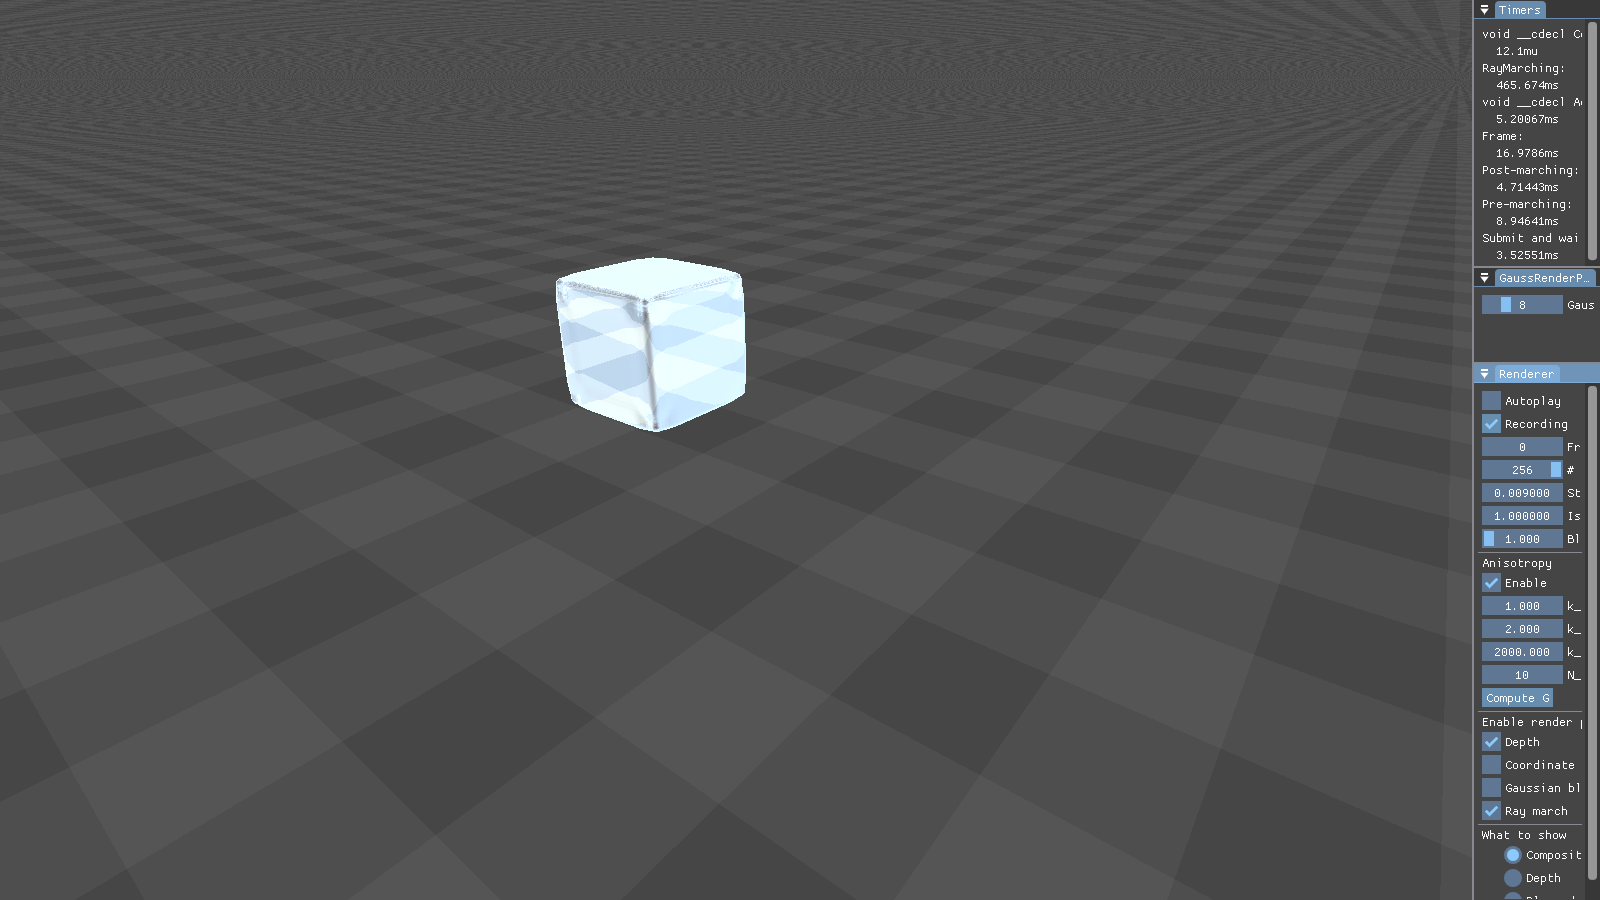
\includegraphics[width=\textwidth]{my-gfx/figure-result-1.png}  
    \end{subfigure}
    \hfill
    \begin{subfigure}[b]{0.475\textwidth}  
        \centering 
        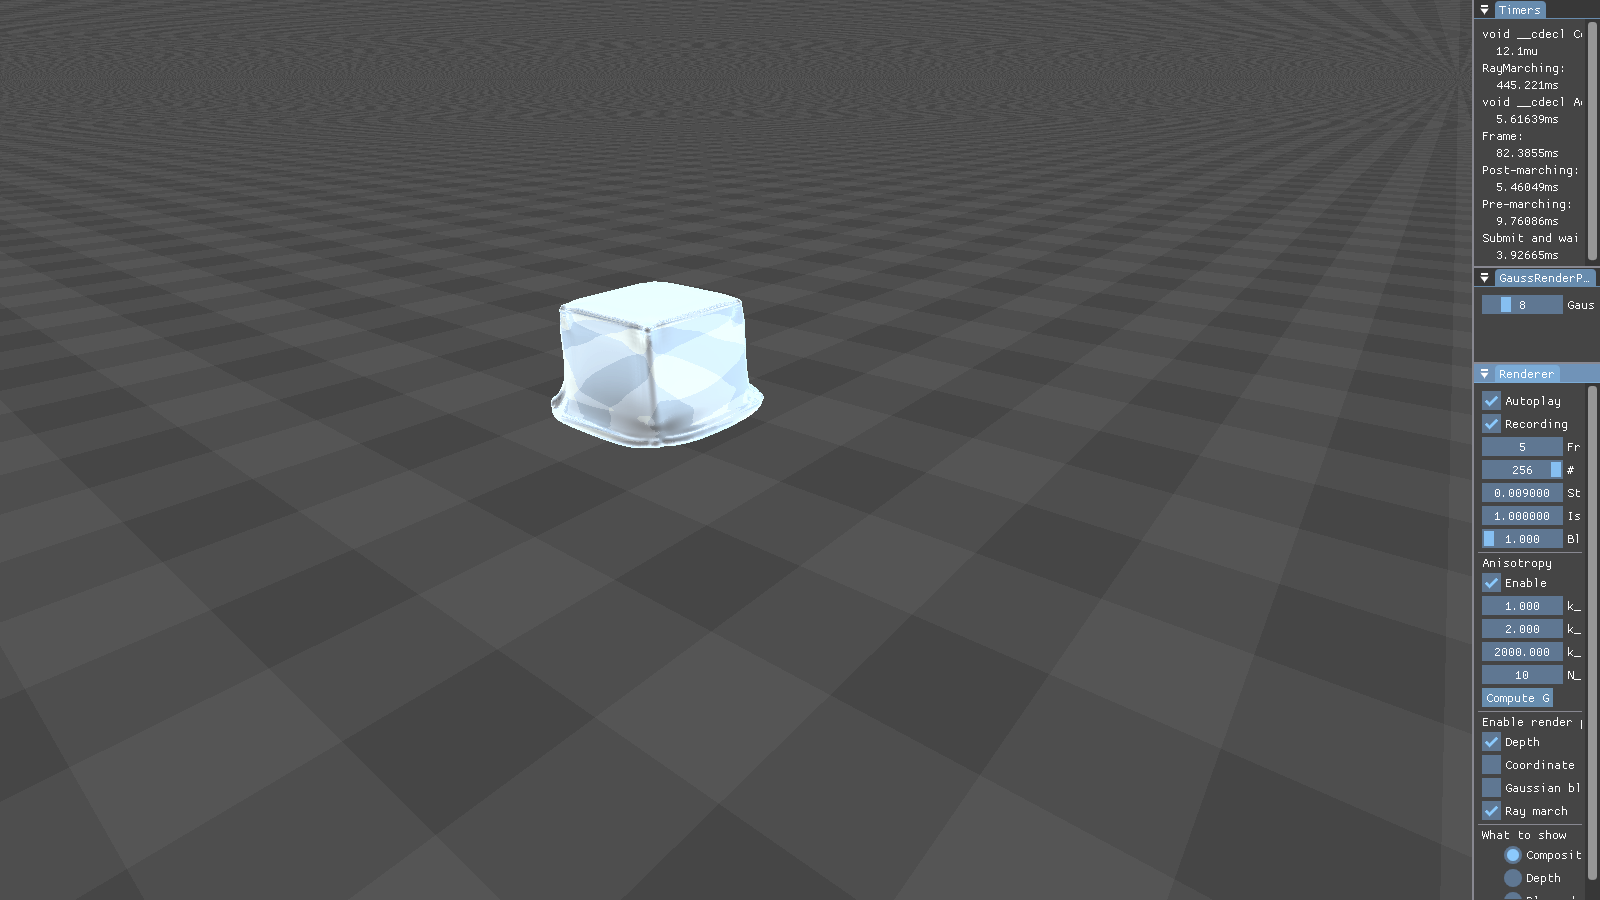
\includegraphics[width=\textwidth]{my-gfx/figure-result-2.png} 
    \end{subfigure}
    \vskip\baselineskip
    \begin{subfigure}[b]{0.475\textwidth}   
        \centering 
        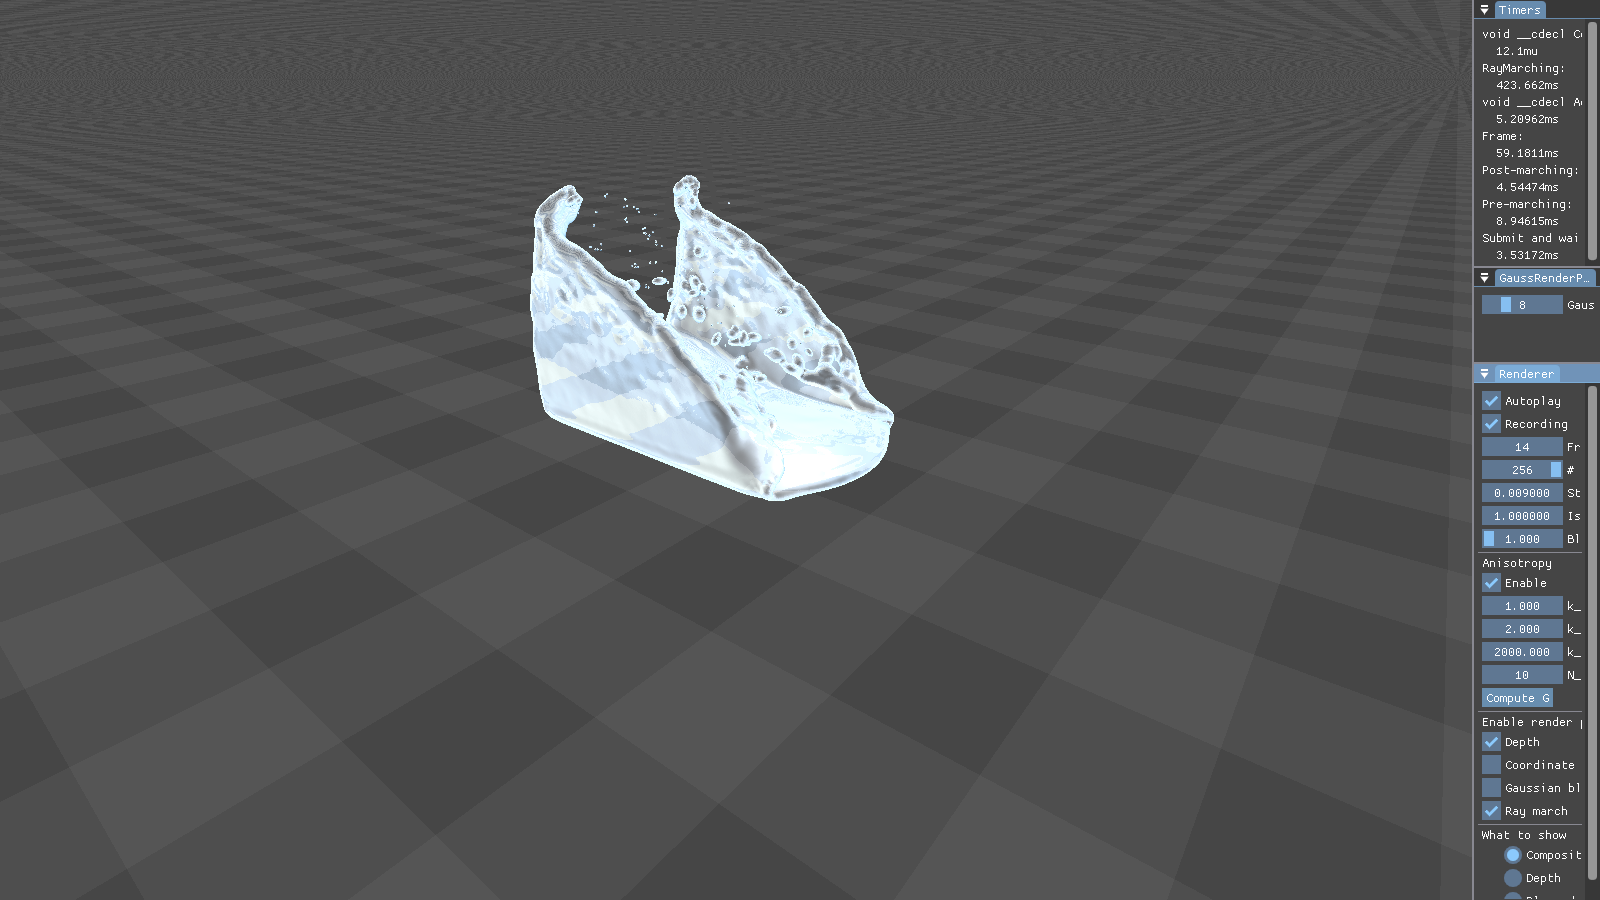
\includegraphics[width=\textwidth]{my-gfx/figure-result-3.png}  
    \end{subfigure}
    \hfill
    \begin{subfigure}[b]{0.475\textwidth}   
        \centering 
        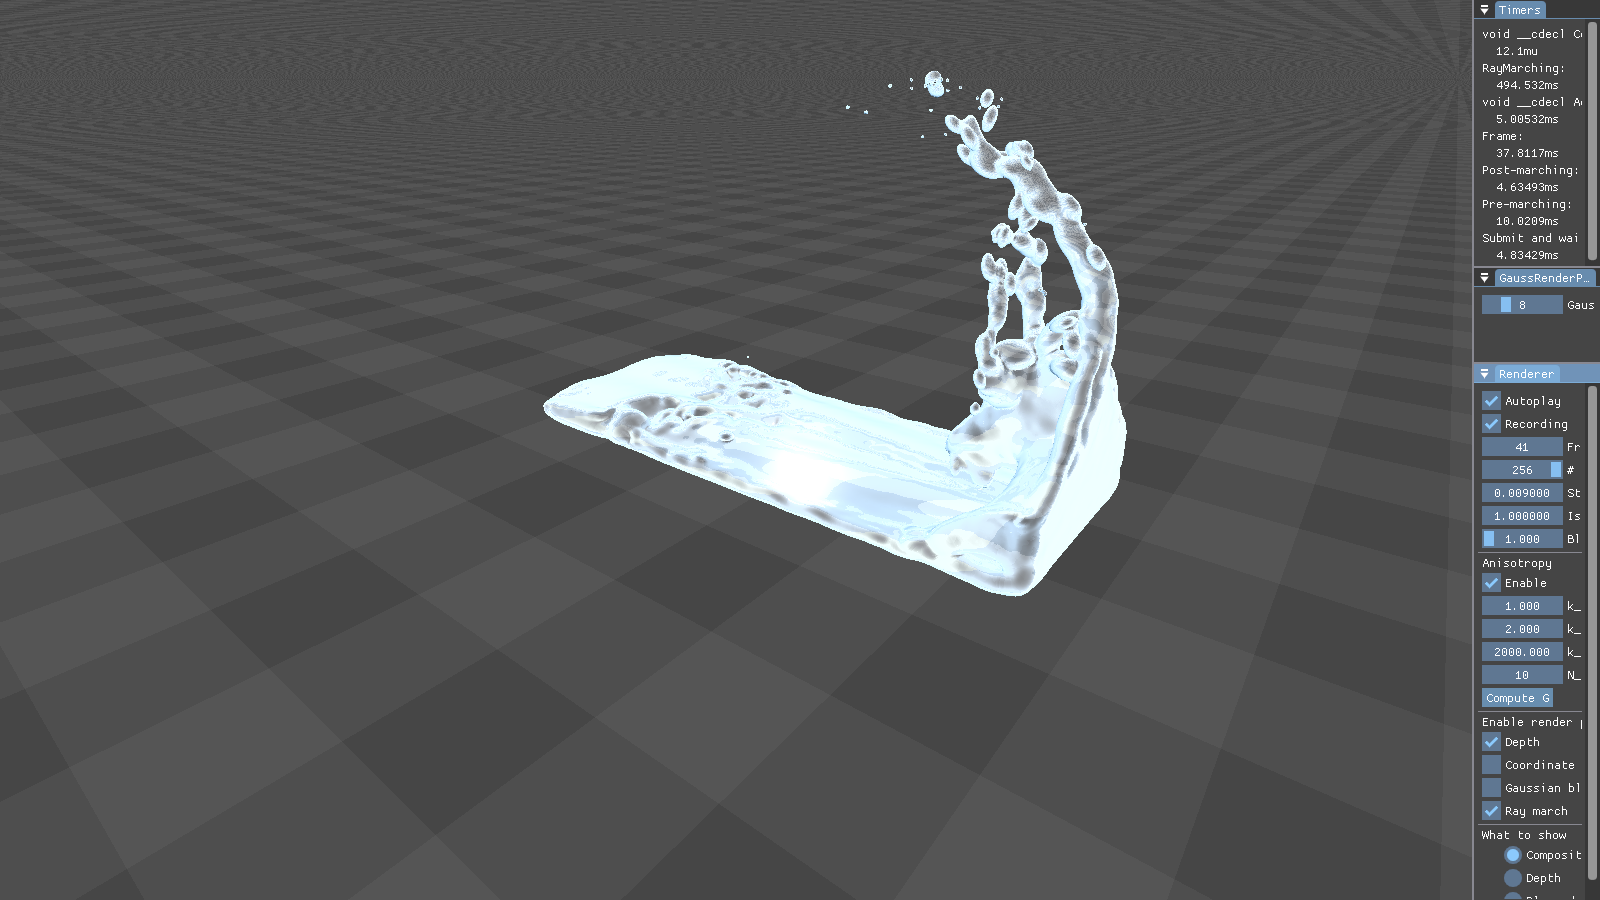
\includegraphics[width=\textwidth]{my-gfx/figure-result-4.png}
    \end{subfigure}
    
    \caption{Four snapshots of our visualization: A cube of fluid dropping into a box.}
    \label{fig:results}
\end{figure*}

Figure \myref{fig:results} shows the results our implementation can produce. Although the particles are spherical by nature, the flat faces of the initial cube configuration still appear to be flat. Particles close to each other merge into threads of fluid, creating a connected surface. Refraction, specularity, and a bluish tinge round off the illusion of water.

With many configurable parameters, the algorithm is very versatile and can be applied to all kinds of fluids. For example, Wu et al. show chocolate running down a model of a bunny in Figure 10 of their paper.

Timing tests were performed on a specific frame of the dam break dataset using a $1600 \times 900$ screen. The exact parameters like the camera position can be extracted from the code repository. The tests ran on an AMD Ryzen 7 1700X 8-core processor and an NVIDIA GeForce GTX 1060 graphics card. On average, the ray marching took $385\text{ms}$ with adaptive step lengths and $404\text{ms}$ with equal step lengths. For this specific scenario, a speedup of around $1.05$ was measured. Note that there are still significant improvements to be achieved when using the techniques Wu et al. propose.

%% !TEX root = ../my-thesis.tex
%
\chapter{Future work}
\label{sec:futurework}

\section{Performance}

Our focus was implementing a working version of the proposed algorithms. Thus, there is a lot of room for improvement of the program's performance. The main source of performance gains will be employing the GPU. Almost every aspect of the algorithm can be implemented in some kind of shader program that the GPU can run in parallel thousands of times: computation of $\textbf{G}_i$ and ray marching iterations to name just a few. It is even possible to execute parts of the pipeline in parallel: Because no neighborhood search has to be performed in the depth pass, it can be executed in tandem with the pre-processing step. \textit{Vulkan} enables a lot of customization, especially for the synchronization of parallel work, making it a natural fit for this application.

\section{Data structure}

Currently, we use multiple separate data structures for neighborhood search and the density grid. It may be beneficial to design a single structure capable of all these features. If the underlying simulation is compatible, simulation and visualization could even share the same structures so they do not have to be rebuilt multiple times per frame.

\section{Multisampling}

The images generated by our algorithm show signs of aliasing. There is a harsh edge between pixels belonging to the fluid and pixels belonging to the background. In computer graphics, a common method of mitigating this is called multi-sampling. For each pixel, multiple samples of the scene are recorded in close proximity and averaged into a single value. This can be achieved by rendering the scene to an image with higher dimensions than the screen and then downsampling it to fit. In our case, this would only have to be done to the composition image. The position and normal buffer could be linearly interpolated between pixels, keeping the ray marching phase unchanged.

\section{Additional fluid features}

Fluids can have many more features than merely color, opacity, reflection et cetera. For example, Ihmsen et al. \cite{Ihmsen:2012} propose a method for displaying foam and bubbles, contributing to the realism of the visualization.
Another crucial part of rendering is shadows. This is prominently achieved with a technique called shadow mapping. The scene is rendered from the perspective of a source of light. For this step, a more lightweight algorithm can be used: Instead of ray marching to find the exact surface position, a smoothed version of the primary depth buffer can be used as a good approximation.
Green \cite{Green:2010} suggests to render the thickness of the fluid to a texture which can be used during image composition to assign dense regions a more opaque color. This models the physical property of molecules scattering light away from the viewers eyes while it travels through a medium.


%% !TEX root = ../my-thesis.tex
%
\chapter{Conclusion}
\label{sec:conclusion}

Wu et al. built on top of existing algorithms for screen-space surface extraction and rendering. They proposed new techniques to accelerate those algorithms and to improve the quality of the result.
These consist of
\begin{enumerate}
    \item adaptive step lengths, reducing the number of iterations for each ray,
    \item adaptive resolution, reducing the number of rays generated,
    \item and adaptively blending normals, enhancing the lighting quality.
\end{enumerate}

They gave little information on their implementation details. Hence, a lot of gaps had to be filled to construct a program capable of rendering fluid surfaces. To see a result on the screen, acceleration structures have to be built using hash grids and maximum density approximation. Depth buffers are filled from which the ray marcher can determine per-pixel information about the surface's position and orientation. Finally, the fluid can be brought to the screen by calculating lighting, transparency, and reflection.

There is no limit when it comes to the visualization of fluids and we are excited to see researchers develop new and improved ways to create beautiful images of them.


% --------------------------
% Back matter
% --------------------------
%
{%
\setstretch{1.1}
\renewcommand{\bibfont}{\normalfont\small}
\setlength{\biblabelsep}{0pt}
\setlength{\bibitemsep}{0.5\baselineskip plus 0.5\baselineskip}
\printbibliography[nottype=online]
\newrefcontext[labelprefix={@}]
\printbibliography[heading=subbibliography,title={Webpages},type=online]
}
\cleardoublepage

\listoffigures
\cleardoublepage

\lstlistoflistings
\cleardoublepage

\appendix\cleardoublepage
%\input{content/chapter-appendix}       % INCLUDE: appendix

\cleardoublepage
\input{content/colophon}

\cleardoublepage
\input{content/declaration}
\clearpage

\newpage
\mbox{}

% **************************************************
% End of Document CONTENT
% **************************************************
\end{document}
